%
% einleitung.tex -- Beispiel-File für die Einleitung
%
% (c) 2020 Prof Dr Andreas Müller, Hochschule Rapperswil
%
\subsection{AM --- Amplitudenmodulation\label{fm:section:teil0}}
\rhead{Amplitudenmodulation}
\begin{figure}
	\centering
	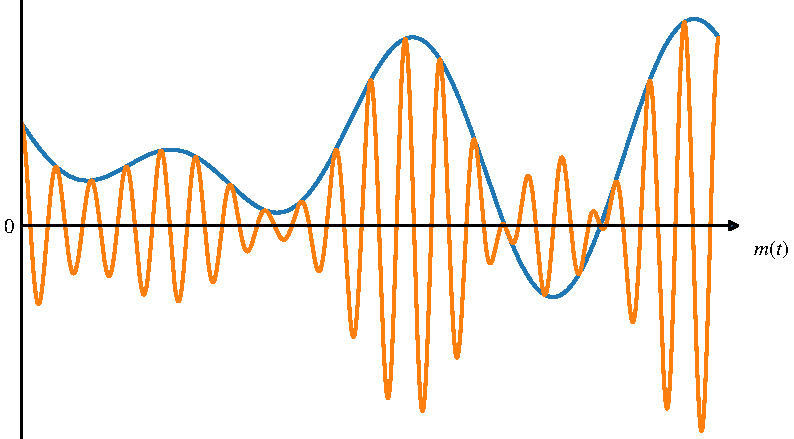
\includegraphics{papers/fm/images/amnormal.pdf}
	%%% Creator: Matplotlib, PGF backend
%%
%% To include the figure in your LaTeX document, write
%%   \input{<filename>.pgf}
%%
%% Make sure the required packages are loaded in your preamble
%%   \usepackage{pgf}
%%
%% Also ensure that all the required font packages are loaded; for instance,
%% the lmodern package is sometimes necessary when using math font.
%%   \usepackage{lmodern}
%%
%% Figures using additional raster images can only be included by \input if
%% they are in the same directory as the main LaTeX file. For loading figures
%% from other directories you can use the `import` package
%%   \usepackage{import}
%%
%% and then include the figures with
%%   \import{<path to file>}{<filename>.pgf}
%%
%% Matplotlib used the following preamble
%%
\begingroup%
\makeatletter%
\begin{pgfpicture}%
\pgfpathrectangle{\pgfpointorigin}{\pgfqpoint{6.000000in}{4.000000in}}%
\pgfusepath{use as bounding box, clip}%
\begin{pgfscope}%
\pgfsetbuttcap%
\pgfsetmiterjoin%
\pgfsetlinewidth{0.000000pt}%
\definecolor{currentstroke}{rgb}{1.000000,1.000000,1.000000}%
\pgfsetstrokecolor{currentstroke}%
\pgfsetstrokeopacity{0.000000}%
\pgfsetdash{}{0pt}%
\pgfpathmoveto{\pgfqpoint{0.000000in}{0.000000in}}%
\pgfpathlineto{\pgfqpoint{6.000000in}{0.000000in}}%
\pgfpathlineto{\pgfqpoint{6.000000in}{4.000000in}}%
\pgfpathlineto{\pgfqpoint{0.000000in}{4.000000in}}%
\pgfpathlineto{\pgfqpoint{0.000000in}{0.000000in}}%
\pgfpathclose%
\pgfusepath{}%
\end{pgfscope}%
\begin{pgfscope}%
\pgfsetbuttcap%
\pgfsetmiterjoin%
\definecolor{currentfill}{rgb}{1.000000,1.000000,1.000000}%
\pgfsetfillcolor{currentfill}%
\pgfsetlinewidth{0.000000pt}%
\definecolor{currentstroke}{rgb}{0.000000,0.000000,0.000000}%
\pgfsetstrokecolor{currentstroke}%
\pgfsetstrokeopacity{0.000000}%
\pgfsetdash{}{0pt}%
\pgfpathmoveto{\pgfqpoint{0.750000in}{0.500000in}}%
\pgfpathlineto{\pgfqpoint{5.400000in}{0.500000in}}%
\pgfpathlineto{\pgfqpoint{5.400000in}{3.520000in}}%
\pgfpathlineto{\pgfqpoint{0.750000in}{3.520000in}}%
\pgfpathlineto{\pgfqpoint{0.750000in}{0.500000in}}%
\pgfpathclose%
\pgfusepath{fill}%
\end{pgfscope}%
\begin{pgfscope}%
\pgfpathrectangle{\pgfqpoint{0.750000in}{0.500000in}}{\pgfqpoint{4.650000in}{3.020000in}}%
\pgfusepath{clip}%
\pgfsetrectcap%
\pgfsetroundjoin%
\pgfsetlinewidth{1.505625pt}%
\definecolor{currentstroke}{rgb}{0.121569,0.466667,0.705882}%
\pgfsetstrokecolor{currentstroke}%
\pgfsetdash{}{0pt}%
\pgfpathmoveto{\pgfqpoint{0.749993in}{2.686751in}}%
\pgfpathlineto{\pgfqpoint{0.822947in}{2.581567in}}%
\pgfpathlineto{\pgfqpoint{0.871292in}{2.517173in}}%
\pgfpathlineto{\pgfqpoint{0.912204in}{2.467673in}}%
\pgfpathlineto{\pgfqpoint{0.948832in}{2.428081in}}%
\pgfpathlineto{\pgfqpoint{0.982557in}{2.396067in}}%
\pgfpathlineto{\pgfqpoint{1.014162in}{2.370235in}}%
\pgfpathlineto{\pgfqpoint{1.044194in}{2.349605in}}%
\pgfpathlineto{\pgfqpoint{1.073054in}{2.333468in}}%
\pgfpathlineto{\pgfqpoint{1.101110in}{2.321275in}}%
\pgfpathlineto{\pgfqpoint{1.128698in}{2.312624in}}%
\pgfpathlineto{\pgfqpoint{1.156151in}{2.307235in}}%
\pgfpathlineto{\pgfqpoint{1.183839in}{2.304945in}}%
\pgfpathlineto{\pgfqpoint{1.212163in}{2.305713in}}%
\pgfpathlineto{\pgfqpoint{1.241604in}{2.309629in}}%
\pgfpathlineto{\pgfqpoint{1.272751in}{2.316931in}}%
\pgfpathlineto{\pgfqpoint{1.306455in}{2.328067in}}%
\pgfpathlineto{\pgfqpoint{1.344131in}{2.343857in}}%
\pgfpathlineto{\pgfqpoint{1.388838in}{2.366089in}}%
\pgfpathlineto{\pgfqpoint{1.452774in}{2.401712in}}%
\pgfpathlineto{\pgfqpoint{1.548013in}{2.454505in}}%
\pgfpathlineto{\pgfqpoint{1.594193in}{2.476379in}}%
\pgfpathlineto{\pgfqpoint{1.633142in}{2.491491in}}%
\pgfpathlineto{\pgfqpoint{1.668218in}{2.501847in}}%
\pgfpathlineto{\pgfqpoint{1.700894in}{2.508319in}}%
\pgfpathlineto{\pgfqpoint{1.732042in}{2.511368in}}%
\pgfpathlineto{\pgfqpoint{1.762274in}{2.511239in}}%
\pgfpathlineto{\pgfqpoint{1.792094in}{2.508024in}}%
\pgfpathlineto{\pgfqpoint{1.821947in}{2.501689in}}%
\pgfpathlineto{\pgfqpoint{1.852280in}{2.492070in}}%
\pgfpathlineto{\pgfqpoint{1.883550in}{2.478876in}}%
\pgfpathlineto{\pgfqpoint{1.916305in}{2.461651in}}%
\pgfpathlineto{\pgfqpoint{1.951269in}{2.439706in}}%
\pgfpathlineto{\pgfqpoint{1.989548in}{2.411940in}}%
\pgfpathlineto{\pgfqpoint{2.033284in}{2.376265in}}%
\pgfpathlineto{\pgfqpoint{2.088616in}{2.326884in}}%
\pgfpathlineto{\pgfqpoint{2.237145in}{2.192211in}}%
\pgfpathlineto{\pgfqpoint{2.278671in}{2.160013in}}%
\pgfpathlineto{\pgfqpoint{2.314082in}{2.136353in}}%
\pgfpathlineto{\pgfqpoint{2.345698in}{2.118852in}}%
\pgfpathlineto{\pgfqpoint{2.374658in}{2.106276in}}%
\pgfpathlineto{\pgfqpoint{2.401688in}{2.097847in}}%
\pgfpathlineto{\pgfqpoint{2.427311in}{2.093049in}}%
\pgfpathlineto{\pgfqpoint{2.451942in}{2.091553in}}%
\pgfpathlineto{\pgfqpoint{2.475947in}{2.093177in}}%
\pgfpathlineto{\pgfqpoint{2.499662in}{2.097880in}}%
\pgfpathlineto{\pgfqpoint{2.523388in}{2.105753in}}%
\pgfpathlineto{\pgfqpoint{2.547416in}{2.117013in}}%
\pgfpathlineto{\pgfqpoint{2.572001in}{2.131995in}}%
\pgfpathlineto{\pgfqpoint{2.597401in}{2.151152in}}%
\pgfpathlineto{\pgfqpoint{2.623873in}{2.175061in}}%
\pgfpathlineto{\pgfqpoint{2.651684in}{2.204431in}}%
\pgfpathlineto{\pgfqpoint{2.681157in}{2.240152in}}%
\pgfpathlineto{\pgfqpoint{2.712684in}{2.283335in}}%
\pgfpathlineto{\pgfqpoint{2.746834in}{2.335485in}}%
\pgfpathlineto{\pgfqpoint{2.784510in}{2.398825in}}%
\pgfpathlineto{\pgfqpoint{2.827398in}{2.477189in}}%
\pgfpathlineto{\pgfqpoint{2.879672in}{2.579485in}}%
\pgfpathlineto{\pgfqpoint{2.969242in}{2.762964in}}%
\pgfpathlineto{\pgfqpoint{3.041682in}{2.908138in}}%
\pgfpathlineto{\pgfqpoint{3.088509in}{2.995243in}}%
\pgfpathlineto{\pgfqpoint{3.127190in}{3.060898in}}%
\pgfpathlineto{\pgfqpoint{3.160982in}{3.112369in}}%
\pgfpathlineto{\pgfqpoint{3.191282in}{3.153067in}}%
\pgfpathlineto{\pgfqpoint{3.218881in}{3.185119in}}%
\pgfpathlineto{\pgfqpoint{3.244281in}{3.210019in}}%
\pgfpathlineto{\pgfqpoint{3.267862in}{3.228927in}}%
\pgfpathlineto{\pgfqpoint{3.289936in}{3.242765in}}%
\pgfpathlineto{\pgfqpoint{3.310795in}{3.252273in}}%
\pgfpathlineto{\pgfqpoint{3.330715in}{3.258016in}}%
\pgfpathlineto{\pgfqpoint{3.350000in}{3.260395in}}%
\pgfpathlineto{\pgfqpoint{3.368938in}{3.259632in}}%
\pgfpathlineto{\pgfqpoint{3.387843in}{3.255767in}}%
\pgfpathlineto{\pgfqpoint{3.406983in}{3.248670in}}%
\pgfpathlineto{\pgfqpoint{3.426636in}{3.238037in}}%
\pgfpathlineto{\pgfqpoint{3.447036in}{3.223416in}}%
\pgfpathlineto{\pgfqpoint{3.468396in}{3.204221in}}%
\pgfpathlineto{\pgfqpoint{3.490928in}{3.179718in}}%
\pgfpathlineto{\pgfqpoint{3.514833in}{3.149040in}}%
\pgfpathlineto{\pgfqpoint{3.540323in}{3.111170in}}%
\pgfpathlineto{\pgfqpoint{3.567665in}{3.064864in}}%
\pgfpathlineto{\pgfqpoint{3.597183in}{3.008628in}}%
\pgfpathlineto{\pgfqpoint{3.629335in}{2.940536in}}%
\pgfpathlineto{\pgfqpoint{3.664857in}{2.857849in}}%
\pgfpathlineto{\pgfqpoint{3.705011in}{2.756281in}}%
\pgfpathlineto{\pgfqpoint{3.752575in}{2.627181in}}%
\pgfpathlineto{\pgfqpoint{3.817326in}{2.441685in}}%
\pgfpathlineto{\pgfqpoint{3.941202in}{2.085603in}}%
\pgfpathlineto{\pgfqpoint{3.989246in}{1.958004in}}%
\pgfpathlineto{\pgfqpoint{4.029087in}{1.860651in}}%
\pgfpathlineto{\pgfqpoint{4.063962in}{1.783318in}}%
\pgfpathlineto{\pgfqpoint{4.095277in}{1.721153in}}%
\pgfpathlineto{\pgfqpoint{4.123780in}{1.671219in}}%
\pgfpathlineto{\pgfqpoint{4.149961in}{1.631388in}}%
\pgfpathlineto{\pgfqpoint{4.174156in}{1.600029in}}%
\pgfpathlineto{\pgfqpoint{4.196632in}{1.575801in}}%
\pgfpathlineto{\pgfqpoint{4.217613in}{1.557595in}}%
\pgfpathlineto{\pgfqpoint{4.237333in}{1.544462in}}%
\pgfpathlineto{\pgfqpoint{4.256026in}{1.535641in}}%
\pgfpathlineto{\pgfqpoint{4.273949in}{1.530541in}}%
\pgfpathlineto{\pgfqpoint{4.291381in}{1.528762in}}%
\pgfpathlineto{\pgfqpoint{4.308623in}{1.530101in}}%
\pgfpathlineto{\pgfqpoint{4.325999in}{1.534571in}}%
\pgfpathlineto{\pgfqpoint{4.343789in}{1.542383in}}%
\pgfpathlineto{\pgfqpoint{4.362258in}{1.553934in}}%
\pgfpathlineto{\pgfqpoint{4.381643in}{1.569784in}}%
\pgfpathlineto{\pgfqpoint{4.402167in}{1.590657in}}%
\pgfpathlineto{\pgfqpoint{4.424029in}{1.617419in}}%
\pgfpathlineto{\pgfqpoint{4.447443in}{1.651102in}}%
\pgfpathlineto{\pgfqpoint{4.472631in}{1.692906in}}%
\pgfpathlineto{\pgfqpoint{4.499873in}{1.744279in}}%
\pgfpathlineto{\pgfqpoint{4.529547in}{1.807031in}}%
\pgfpathlineto{\pgfqpoint{4.562201in}{1.883533in}}%
\pgfpathlineto{\pgfqpoint{4.598728in}{1.977239in}}%
\pgfpathlineto{\pgfqpoint{4.640824in}{2.094069in}}%
\pgfpathlineto{\pgfqpoint{4.692718in}{2.247720in}}%
\pgfpathlineto{\pgfqpoint{4.781116in}{2.521031in}}%
\pgfpathlineto{\pgfqpoint{4.857696in}{2.753518in}}%
\pgfpathlineto{\pgfqpoint{4.906745in}{2.892766in}}%
\pgfpathlineto{\pgfqpoint{4.947490in}{2.999463in}}%
\pgfpathlineto{\pgfqpoint{4.983280in}{3.084805in}}%
\pgfpathlineto{\pgfqpoint{5.015521in}{3.153947in}}%
\pgfpathlineto{\pgfqpoint{5.044984in}{3.210045in}}%
\pgfpathlineto{\pgfqpoint{5.072147in}{3.255323in}}%
\pgfpathlineto{\pgfqpoint{5.097336in}{3.291486in}}%
\pgfpathlineto{\pgfqpoint{5.120805in}{3.319940in}}%
\pgfpathlineto{\pgfqpoint{5.142779in}{3.341870in}}%
\pgfpathlineto{\pgfqpoint{5.163459in}{3.358265in}}%
\pgfpathlineto{\pgfqpoint{5.183056in}{3.369958in}}%
\pgfpathlineto{\pgfqpoint{5.201805in}{3.377621in}}%
\pgfpathlineto{\pgfqpoint{5.219962in}{3.381750in}}%
\pgfpathlineto{\pgfqpoint{5.237807in}{3.382660in}}%
\pgfpathlineto{\pgfqpoint{5.255640in}{3.380470in}}%
\pgfpathlineto{\pgfqpoint{5.273753in}{3.375106in}}%
\pgfpathlineto{\pgfqpoint{5.292446in}{3.366299in}}%
\pgfpathlineto{\pgfqpoint{5.311987in}{3.353609in}}%
\pgfpathlineto{\pgfqpoint{5.332622in}{3.336438in}}%
\pgfpathlineto{\pgfqpoint{5.354596in}{3.314029in}}%
\pgfpathlineto{\pgfqpoint{5.378155in}{3.285469in}}%
\pgfpathlineto{\pgfqpoint{5.400007in}{3.254987in}}%
\pgfpathlineto{\pgfqpoint{5.400007in}{3.254987in}}%
\pgfusepath{stroke}%
\end{pgfscope}%
\begin{pgfscope}%
\pgfpathrectangle{\pgfqpoint{0.750000in}{0.500000in}}{\pgfqpoint{4.650000in}{3.020000in}}%
\pgfusepath{clip}%
\pgfsetrectcap%
\pgfsetroundjoin%
\pgfsetlinewidth{1.505625pt}%
\definecolor{currentstroke}{rgb}{1.000000,0.498039,0.054902}%
\pgfsetstrokecolor{currentstroke}%
\pgfsetdash{}{0pt}%
\pgfpathmoveto{\pgfqpoint{0.749993in}{2.686751in}}%
\pgfpathlineto{\pgfqpoint{0.753330in}{2.679074in}}%
\pgfpathlineto{\pgfqpoint{0.757928in}{2.659689in}}%
\pgfpathlineto{\pgfqpoint{0.764022in}{2.619100in}}%
\pgfpathlineto{\pgfqpoint{0.771934in}{2.543506in}}%
\pgfpathlineto{\pgfqpoint{0.782391in}{2.411036in}}%
\pgfpathlineto{\pgfqpoint{0.798294in}{2.164838in}}%
\pgfpathlineto{\pgfqpoint{0.825859in}{1.739669in}}%
\pgfpathlineto{\pgfqpoint{0.837711in}{1.604541in}}%
\pgfpathlineto{\pgfqpoint{0.846829in}{1.532484in}}%
\pgfpathlineto{\pgfqpoint{0.853949in}{1.497891in}}%
\pgfpathlineto{\pgfqpoint{0.859295in}{1.484884in}}%
\pgfpathlineto{\pgfqpoint{0.862978in}{1.482404in}}%
\pgfpathlineto{\pgfqpoint{0.865823in}{1.484062in}}%
\pgfpathlineto{\pgfqpoint{0.869350in}{1.490353in}}%
\pgfpathlineto{\pgfqpoint{0.874104in}{1.506016in}}%
\pgfpathlineto{\pgfqpoint{0.880354in}{1.538420in}}%
\pgfpathlineto{\pgfqpoint{0.888467in}{1.598413in}}%
\pgfpathlineto{\pgfqpoint{0.899236in}{1.703331in}}%
\pgfpathlineto{\pgfqpoint{0.916177in}{1.903228in}}%
\pgfpathlineto{\pgfqpoint{0.941444in}{2.196187in}}%
\pgfpathlineto{\pgfqpoint{0.953519in}{2.301217in}}%
\pgfpathlineto{\pgfqpoint{0.962804in}{2.357532in}}%
\pgfpathlineto{\pgfqpoint{0.970080in}{2.384887in}}%
\pgfpathlineto{\pgfqpoint{0.975605in}{2.395406in}}%
\pgfpathlineto{\pgfqpoint{0.979577in}{2.397485in}}%
\pgfpathlineto{\pgfqpoint{0.982870in}{2.395772in}}%
\pgfpathlineto{\pgfqpoint{0.986820in}{2.389699in}}%
\pgfpathlineto{\pgfqpoint{0.991987in}{2.375380in}}%
\pgfpathlineto{\pgfqpoint{0.998683in}{2.346764in}}%
\pgfpathlineto{\pgfqpoint{1.007321in}{2.295009in}}%
\pgfpathlineto{\pgfqpoint{1.018883in}{2.205120in}}%
\pgfpathlineto{\pgfqpoint{1.038815in}{2.021157in}}%
\pgfpathlineto{\pgfqpoint{1.059807in}{1.837455in}}%
\pgfpathlineto{\pgfqpoint{1.071849in}{1.757548in}}%
\pgfpathlineto{\pgfqpoint{1.081089in}{1.714946in}}%
\pgfpathlineto{\pgfqpoint{1.088310in}{1.694525in}}%
\pgfpathlineto{\pgfqpoint{1.093811in}{1.686921in}}%
\pgfpathlineto{\pgfqpoint{1.097907in}{1.685781in}}%
\pgfpathlineto{\pgfqpoint{1.101623in}{1.688063in}}%
\pgfpathlineto{\pgfqpoint{1.106087in}{1.694900in}}%
\pgfpathlineto{\pgfqpoint{1.111801in}{1.709954in}}%
\pgfpathlineto{\pgfqpoint{1.119078in}{1.738707in}}%
\pgfpathlineto{\pgfqpoint{1.128363in}{1.789143in}}%
\pgfpathlineto{\pgfqpoint{1.140817in}{1.875538in}}%
\pgfpathlineto{\pgfqpoint{1.167981in}{2.093317in}}%
\pgfpathlineto{\pgfqpoint{1.183873in}{2.204633in}}%
\pgfpathlineto{\pgfqpoint{1.194776in}{2.261064in}}%
\pgfpathlineto{\pgfqpoint{1.203146in}{2.289824in}}%
\pgfpathlineto{\pgfqpoint{1.209586in}{2.302297in}}%
\pgfpathlineto{\pgfqpoint{1.214384in}{2.305859in}}%
\pgfpathlineto{\pgfqpoint{1.218201in}{2.305136in}}%
\pgfpathlineto{\pgfqpoint{1.222286in}{2.300867in}}%
\pgfpathlineto{\pgfqpoint{1.227386in}{2.290527in}}%
\pgfpathlineto{\pgfqpoint{1.233836in}{2.269732in}}%
\pgfpathlineto{\pgfqpoint{1.241938in}{2.232225in}}%
\pgfpathlineto{\pgfqpoint{1.252273in}{2.168452in}}%
\pgfpathlineto{\pgfqpoint{1.266636in}{2.058386in}}%
\pgfpathlineto{\pgfqpoint{1.303397in}{1.768481in}}%
\pgfpathlineto{\pgfqpoint{1.314021in}{1.712010in}}%
\pgfpathlineto{\pgfqpoint{1.322079in}{1.684052in}}%
\pgfpathlineto{\pgfqpoint{1.328172in}{1.672557in}}%
\pgfpathlineto{\pgfqpoint{1.332625in}{1.669717in}}%
\pgfpathlineto{\pgfqpoint{1.336196in}{1.670915in}}%
\pgfpathlineto{\pgfqpoint{1.340191in}{1.675947in}}%
\pgfpathlineto{\pgfqpoint{1.345258in}{1.687907in}}%
\pgfpathlineto{\pgfqpoint{1.351675in}{1.711795in}}%
\pgfpathlineto{\pgfqpoint{1.359732in}{1.754804in}}%
\pgfpathlineto{\pgfqpoint{1.369966in}{1.827703in}}%
\pgfpathlineto{\pgfqpoint{1.384095in}{1.952972in}}%
\pgfpathlineto{\pgfqpoint{1.421034in}{2.290666in}}%
\pgfpathlineto{\pgfqpoint{1.431391in}{2.353569in}}%
\pgfpathlineto{\pgfqpoint{1.439214in}{2.384228in}}%
\pgfpathlineto{\pgfqpoint{1.445073in}{2.396459in}}%
\pgfpathlineto{\pgfqpoint{1.449247in}{2.399251in}}%
\pgfpathlineto{\pgfqpoint{1.452506in}{2.397927in}}%
\pgfpathlineto{\pgfqpoint{1.456267in}{2.392551in}}%
\pgfpathlineto{\pgfqpoint{1.461132in}{2.379503in}}%
\pgfpathlineto{\pgfqpoint{1.467360in}{2.352995in}}%
\pgfpathlineto{\pgfqpoint{1.475205in}{2.304791in}}%
\pgfpathlineto{\pgfqpoint{1.485171in}{2.222591in}}%
\pgfpathlineto{\pgfqpoint{1.498809in}{2.081734in}}%
\pgfpathlineto{\pgfqpoint{1.537768in}{1.664278in}}%
\pgfpathlineto{\pgfqpoint{1.547812in}{1.594915in}}%
\pgfpathlineto{\pgfqpoint{1.555423in}{1.561387in}}%
\pgfpathlineto{\pgfqpoint{1.561093in}{1.548303in}}%
\pgfpathlineto{\pgfqpoint{1.565055in}{1.545476in}}%
\pgfpathlineto{\pgfqpoint{1.568079in}{1.546878in}}%
\pgfpathlineto{\pgfqpoint{1.571650in}{1.552518in}}%
\pgfpathlineto{\pgfqpoint{1.576360in}{1.566512in}}%
\pgfpathlineto{\pgfqpoint{1.582442in}{1.595351in}}%
\pgfpathlineto{\pgfqpoint{1.590142in}{1.648266in}}%
\pgfpathlineto{\pgfqpoint{1.599974in}{1.739237in}}%
\pgfpathlineto{\pgfqpoint{1.613456in}{1.895778in}}%
\pgfpathlineto{\pgfqpoint{1.652772in}{2.369997in}}%
\pgfpathlineto{\pgfqpoint{1.662839in}{2.448046in}}%
\pgfpathlineto{\pgfqpoint{1.670494in}{2.486050in}}%
\pgfpathlineto{\pgfqpoint{1.676220in}{2.501123in}}%
\pgfpathlineto{\pgfqpoint{1.680204in}{2.504587in}}%
\pgfpathlineto{\pgfqpoint{1.683105in}{2.503432in}}%
\pgfpathlineto{\pgfqpoint{1.686498in}{2.498150in}}%
\pgfpathlineto{\pgfqpoint{1.691018in}{2.484590in}}%
\pgfpathlineto{\pgfqpoint{1.696910in}{2.456027in}}%
\pgfpathlineto{\pgfqpoint{1.704421in}{2.402837in}}%
\pgfpathlineto{\pgfqpoint{1.714041in}{2.310603in}}%
\pgfpathlineto{\pgfqpoint{1.727232in}{2.151201in}}%
\pgfpathlineto{\pgfqpoint{1.767899in}{1.638928in}}%
\pgfpathlineto{\pgfqpoint{1.777887in}{1.559265in}}%
\pgfpathlineto{\pgfqpoint{1.785543in}{1.520184in}}%
\pgfpathlineto{\pgfqpoint{1.791291in}{1.504560in}}%
\pgfpathlineto{\pgfqpoint{1.795308in}{1.500862in}}%
\pgfpathlineto{\pgfqpoint{1.798210in}{1.501916in}}%
\pgfpathlineto{\pgfqpoint{1.801569in}{1.507019in}}%
\pgfpathlineto{\pgfqpoint{1.806055in}{1.520240in}}%
\pgfpathlineto{\pgfqpoint{1.811937in}{1.548295in}}%
\pgfpathlineto{\pgfqpoint{1.819470in}{1.600773in}}%
\pgfpathlineto{\pgfqpoint{1.829190in}{1.692239in}}%
\pgfpathlineto{\pgfqpoint{1.842761in}{1.852398in}}%
\pgfpathlineto{\pgfqpoint{1.880437in}{2.312463in}}%
\pgfpathlineto{\pgfqpoint{1.890927in}{2.397460in}}%
\pgfpathlineto{\pgfqpoint{1.899007in}{2.440460in}}%
\pgfpathlineto{\pgfqpoint{1.905167in}{2.458809in}}%
\pgfpathlineto{\pgfqpoint{1.909598in}{2.464033in}}%
\pgfpathlineto{\pgfqpoint{1.912734in}{2.463682in}}%
\pgfpathlineto{\pgfqpoint{1.916037in}{2.459716in}}%
\pgfpathlineto{\pgfqpoint{1.920390in}{2.448964in}}%
\pgfpathlineto{\pgfqpoint{1.926115in}{2.425616in}}%
\pgfpathlineto{\pgfqpoint{1.933492in}{2.381253in}}%
\pgfpathlineto{\pgfqpoint{1.943067in}{2.303045in}}%
\pgfpathlineto{\pgfqpoint{1.956492in}{2.165121in}}%
\pgfpathlineto{\pgfqpoint{1.994347in}{1.762409in}}%
\pgfpathlineto{\pgfqpoint{2.004949in}{1.687457in}}%
\pgfpathlineto{\pgfqpoint{2.013174in}{1.649024in}}%
\pgfpathlineto{\pgfqpoint{2.019524in}{1.632178in}}%
\pgfpathlineto{\pgfqpoint{2.024200in}{1.627089in}}%
\pgfpathlineto{\pgfqpoint{2.027649in}{1.627297in}}%
\pgfpathlineto{\pgfqpoint{2.031220in}{1.630996in}}%
\pgfpathlineto{\pgfqpoint{2.035807in}{1.640798in}}%
\pgfpathlineto{\pgfqpoint{2.041800in}{1.661723in}}%
\pgfpathlineto{\pgfqpoint{2.049545in}{1.701109in}}%
\pgfpathlineto{\pgfqpoint{2.059745in}{1.770529in}}%
\pgfpathlineto{\pgfqpoint{2.075045in}{1.898748in}}%
\pgfpathlineto{\pgfqpoint{2.103782in}{2.140310in}}%
\pgfpathlineto{\pgfqpoint{2.115489in}{2.212134in}}%
\pgfpathlineto{\pgfqpoint{2.124551in}{2.250397in}}%
\pgfpathlineto{\pgfqpoint{2.131705in}{2.268729in}}%
\pgfpathlineto{\pgfqpoint{2.137207in}{2.275504in}}%
\pgfpathlineto{\pgfqpoint{2.141425in}{2.276421in}}%
\pgfpathlineto{\pgfqpoint{2.145387in}{2.273985in}}%
\pgfpathlineto{\pgfqpoint{2.150163in}{2.266970in}}%
\pgfpathlineto{\pgfqpoint{2.156279in}{2.251892in}}%
\pgfpathlineto{\pgfqpoint{2.164192in}{2.223344in}}%
\pgfpathlineto{\pgfqpoint{2.174738in}{2.172586in}}%
\pgfpathlineto{\pgfqpoint{2.191567in}{2.074002in}}%
\pgfpathlineto{\pgfqpoint{2.216019in}{1.933779in}}%
\pgfpathlineto{\pgfqpoint{2.228150in}{1.881668in}}%
\pgfpathlineto{\pgfqpoint{2.237624in}{1.853354in}}%
\pgfpathlineto{\pgfqpoint{2.245258in}{1.839280in}}%
\pgfpathlineto{\pgfqpoint{2.251396in}{1.833723in}}%
\pgfpathlineto{\pgfqpoint{2.256507in}{1.832932in}}%
\pgfpathlineto{\pgfqpoint{2.261507in}{1.835390in}}%
\pgfpathlineto{\pgfqpoint{2.267321in}{1.842013in}}%
\pgfpathlineto{\pgfqpoint{2.274598in}{1.855439in}}%
\pgfpathlineto{\pgfqpoint{2.284039in}{1.879954in}}%
\pgfpathlineto{\pgfqpoint{2.297498in}{1.924477in}}%
\pgfpathlineto{\pgfqpoint{2.335609in}{2.055043in}}%
\pgfpathlineto{\pgfqpoint{2.347205in}{2.081988in}}%
\pgfpathlineto{\pgfqpoint{2.356635in}{2.096727in}}%
\pgfpathlineto{\pgfqpoint{2.364536in}{2.103822in}}%
\pgfpathlineto{\pgfqpoint{2.371422in}{2.106113in}}%
\pgfpathlineto{\pgfqpoint{2.377962in}{2.105061in}}%
\pgfpathlineto{\pgfqpoint{2.384993in}{2.100647in}}%
\pgfpathlineto{\pgfqpoint{2.393251in}{2.091549in}}%
\pgfpathlineto{\pgfqpoint{2.403507in}{2.075290in}}%
\pgfpathlineto{\pgfqpoint{2.417301in}{2.047076in}}%
\pgfpathlineto{\pgfqpoint{2.469809in}{1.933586in}}%
\pgfpathlineto{\pgfqpoint{2.480712in}{1.919835in}}%
\pgfpathlineto{\pgfqpoint{2.489540in}{1.913293in}}%
\pgfpathlineto{\pgfqpoint{2.497050in}{1.911353in}}%
\pgfpathlineto{\pgfqpoint{2.503981in}{1.912723in}}%
\pgfpathlineto{\pgfqpoint{2.511112in}{1.917414in}}%
\pgfpathlineto{\pgfqpoint{2.519024in}{1.926554in}}%
\pgfpathlineto{\pgfqpoint{2.528187in}{1.942189in}}%
\pgfpathlineto{\pgfqpoint{2.539146in}{1.967448in}}%
\pgfpathlineto{\pgfqpoint{2.553241in}{2.008383in}}%
\pgfpathlineto{\pgfqpoint{2.597379in}{2.142663in}}%
\pgfpathlineto{\pgfqpoint{2.606419in}{2.158123in}}%
\pgfpathlineto{\pgfqpoint{2.613260in}{2.164372in}}%
\pgfpathlineto{\pgfqpoint{2.618683in}{2.165511in}}%
\pgfpathlineto{\pgfqpoint{2.623638in}{2.163366in}}%
\pgfpathlineto{\pgfqpoint{2.629051in}{2.157374in}}%
\pgfpathlineto{\pgfqpoint{2.635435in}{2.145273in}}%
\pgfpathlineto{\pgfqpoint{2.643090in}{2.123558in}}%
\pgfpathlineto{\pgfqpoint{2.652353in}{2.087235in}}%
\pgfpathlineto{\pgfqpoint{2.663993in}{2.028019in}}%
\pgfpathlineto{\pgfqpoint{2.681347in}{1.921447in}}%
\pgfpathlineto{\pgfqpoint{2.705330in}{1.777186in}}%
\pgfpathlineto{\pgfqpoint{2.716055in}{1.730668in}}%
\pgfpathlineto{\pgfqpoint{2.723844in}{1.709029in}}%
\pgfpathlineto{\pgfqpoint{2.729569in}{1.700962in}}%
\pgfpathlineto{\pgfqpoint{2.733721in}{1.699672in}}%
\pgfpathlineto{\pgfqpoint{2.737359in}{1.701858in}}%
\pgfpathlineto{\pgfqpoint{2.741633in}{1.708510in}}%
\pgfpathlineto{\pgfqpoint{2.747001in}{1.723237in}}%
\pgfpathlineto{\pgfqpoint{2.753675in}{1.751464in}}%
\pgfpathlineto{\pgfqpoint{2.761889in}{1.800826in}}%
\pgfpathlineto{\pgfqpoint{2.772123in}{1.882743in}}%
\pgfpathlineto{\pgfqpoint{2.785916in}{2.020636in}}%
\pgfpathlineto{\pgfqpoint{2.823503in}{2.409797in}}%
\pgfpathlineto{\pgfqpoint{2.833034in}{2.472161in}}%
\pgfpathlineto{\pgfqpoint{2.840065in}{2.500317in}}%
\pgfpathlineto{\pgfqpoint{2.845109in}{2.509888in}}%
\pgfpathlineto{\pgfqpoint{2.848479in}{2.511009in}}%
\pgfpathlineto{\pgfqpoint{2.851370in}{2.508494in}}%
\pgfpathlineto{\pgfqpoint{2.855075in}{2.500488in}}%
\pgfpathlineto{\pgfqpoint{2.859963in}{2.481616in}}%
\pgfpathlineto{\pgfqpoint{2.866190in}{2.443934in}}%
\pgfpathlineto{\pgfqpoint{2.873958in}{2.376227in}}%
\pgfpathlineto{\pgfqpoint{2.883689in}{2.261914in}}%
\pgfpathlineto{\pgfqpoint{2.896601in}{2.070252in}}%
\pgfpathlineto{\pgfqpoint{2.940148in}{1.391608in}}%
\pgfpathlineto{\pgfqpoint{2.949087in}{1.311025in}}%
\pgfpathlineto{\pgfqpoint{2.955727in}{1.275459in}}%
\pgfpathlineto{\pgfqpoint{2.960426in}{1.264108in}}%
\pgfpathlineto{\pgfqpoint{2.963350in}{1.263095in}}%
\pgfpathlineto{\pgfqpoint{2.965816in}{1.265929in}}%
\pgfpathlineto{\pgfqpoint{2.969209in}{1.275402in}}%
\pgfpathlineto{\pgfqpoint{2.973818in}{1.298658in}}%
\pgfpathlineto{\pgfqpoint{2.979799in}{1.346511in}}%
\pgfpathlineto{\pgfqpoint{2.987332in}{1.434082in}}%
\pgfpathlineto{\pgfqpoint{2.996818in}{1.583605in}}%
\pgfpathlineto{\pgfqpoint{3.009396in}{1.835379in}}%
\pgfpathlineto{\pgfqpoint{3.055409in}{2.807024in}}%
\pgfpathlineto{\pgfqpoint{3.064203in}{2.910900in}}%
\pgfpathlineto{\pgfqpoint{3.070787in}{2.956925in}}%
\pgfpathlineto{\pgfqpoint{3.075430in}{2.971590in}}%
\pgfpathlineto{\pgfqpoint{3.078231in}{2.973054in}}%
\pgfpathlineto{\pgfqpoint{3.080407in}{2.970298in}}%
\pgfpathlineto{\pgfqpoint{3.083532in}{2.960348in}}%
\pgfpathlineto{\pgfqpoint{3.087884in}{2.934720in}}%
\pgfpathlineto{\pgfqpoint{3.093609in}{2.880428in}}%
\pgfpathlineto{\pgfqpoint{3.100886in}{2.779067in}}%
\pgfpathlineto{\pgfqpoint{3.110093in}{2.603781in}}%
\pgfpathlineto{\pgfqpoint{3.122268in}{2.307421in}}%
\pgfpathlineto{\pgfqpoint{3.146162in}{1.629196in}}%
\pgfpathlineto{\pgfqpoint{3.162746in}{1.206891in}}%
\pgfpathlineto{\pgfqpoint{3.173437in}{1.006359in}}%
\pgfpathlineto{\pgfqpoint{3.181472in}{0.907139in}}%
\pgfpathlineto{\pgfqpoint{3.187454in}{0.865974in}}%
\pgfpathlineto{\pgfqpoint{3.191550in}{0.854828in}}%
\pgfpathlineto{\pgfqpoint{3.193815in}{0.854743in}}%
\pgfpathlineto{\pgfqpoint{3.196036in}{0.858896in}}%
\pgfpathlineto{\pgfqpoint{3.199328in}{0.872770in}}%
\pgfpathlineto{\pgfqpoint{3.203904in}{0.907257in}}%
\pgfpathlineto{\pgfqpoint{3.209897in}{0.978530in}}%
\pgfpathlineto{\pgfqpoint{3.217541in}{1.109936in}}%
\pgfpathlineto{\pgfqpoint{3.227306in}{1.335839in}}%
\pgfpathlineto{\pgfqpoint{3.240710in}{1.725017in}}%
\pgfpathlineto{\pgfqpoint{3.280171in}{2.915855in}}%
\pgfpathlineto{\pgfqpoint{3.290193in}{3.109860in}}%
\pgfpathlineto{\pgfqpoint{3.297804in}{3.204351in}}%
\pgfpathlineto{\pgfqpoint{3.303451in}{3.241882in}}%
\pgfpathlineto{\pgfqpoint{3.307223in}{3.250861in}}%
\pgfpathlineto{\pgfqpoint{3.309221in}{3.250330in}}%
\pgfpathlineto{\pgfqpoint{3.311509in}{3.245217in}}%
\pgfpathlineto{\pgfqpoint{3.314913in}{3.228741in}}%
\pgfpathlineto{\pgfqpoint{3.319633in}{3.188571in}}%
\pgfpathlineto{\pgfqpoint{3.325816in}{3.106547in}}%
\pgfpathlineto{\pgfqpoint{3.333728in}{2.956435in}}%
\pgfpathlineto{\pgfqpoint{3.343951in}{2.698363in}}%
\pgfpathlineto{\pgfqpoint{3.358593in}{2.241414in}}%
\pgfpathlineto{\pgfqpoint{3.391013in}{1.211744in}}%
\pgfpathlineto{\pgfqpoint{3.402005in}{0.966501in}}%
\pgfpathlineto{\pgfqpoint{3.410364in}{0.841553in}}%
\pgfpathlineto{\pgfqpoint{3.416703in}{0.786769in}}%
\pgfpathlineto{\pgfqpoint{3.421178in}{0.769849in}}%
\pgfpathlineto{\pgfqpoint{3.423723in}{0.768365in}}%
\pgfpathlineto{\pgfqpoint{3.423779in}{0.768399in}}%
\pgfpathlineto{\pgfqpoint{3.425787in}{0.771497in}}%
\pgfpathlineto{\pgfqpoint{3.428801in}{0.782997in}}%
\pgfpathlineto{\pgfqpoint{3.433086in}{0.813316in}}%
\pgfpathlineto{\pgfqpoint{3.438800in}{0.878419in}}%
\pgfpathlineto{\pgfqpoint{3.446177in}{1.001379in}}%
\pgfpathlineto{\pgfqpoint{3.455707in}{1.216679in}}%
\pgfpathlineto{\pgfqpoint{3.468910in}{1.592323in}}%
\pgfpathlineto{\pgfqpoint{3.508550in}{2.765438in}}%
\pgfpathlineto{\pgfqpoint{3.518784in}{2.961306in}}%
\pgfpathlineto{\pgfqpoint{3.526674in}{3.059740in}}%
\pgfpathlineto{\pgfqpoint{3.532645in}{3.101092in}}%
\pgfpathlineto{\pgfqpoint{3.536785in}{3.112540in}}%
\pgfpathlineto{\pgfqpoint{3.539117in}{3.112762in}}%
\pgfpathlineto{\pgfqpoint{3.541349in}{3.108801in}}%
\pgfpathlineto{\pgfqpoint{3.544664in}{3.095477in}}%
\pgfpathlineto{\pgfqpoint{3.549295in}{3.062320in}}%
\pgfpathlineto{\pgfqpoint{3.555433in}{2.993519in}}%
\pgfpathlineto{\pgfqpoint{3.563379in}{2.866252in}}%
\pgfpathlineto{\pgfqpoint{3.573859in}{2.644058in}}%
\pgfpathlineto{\pgfqpoint{3.589840in}{2.230376in}}%
\pgfpathlineto{\pgfqpoint{3.616568in}{1.543135in}}%
\pgfpathlineto{\pgfqpoint{3.628253in}{1.321405in}}%
\pgfpathlineto{\pgfqpoint{3.637203in}{1.204380in}}%
\pgfpathlineto{\pgfqpoint{3.644144in}{1.149117in}}%
\pgfpathlineto{\pgfqpoint{3.649278in}{1.128943in}}%
\pgfpathlineto{\pgfqpoint{3.652626in}{1.125280in}}%
\pgfpathlineto{\pgfqpoint{3.654791in}{1.126855in}}%
\pgfpathlineto{\pgfqpoint{3.657682in}{1.133707in}}%
\pgfpathlineto{\pgfqpoint{3.661800in}{1.152608in}}%
\pgfpathlineto{\pgfqpoint{3.667368in}{1.194433in}}%
\pgfpathlineto{\pgfqpoint{3.674667in}{1.275079in}}%
\pgfpathlineto{\pgfqpoint{3.684309in}{1.419271in}}%
\pgfpathlineto{\pgfqpoint{3.698371in}{1.681563in}}%
\pgfpathlineto{\pgfqpoint{3.730623in}{2.294745in}}%
\pgfpathlineto{\pgfqpoint{3.741873in}{2.445780in}}%
\pgfpathlineto{\pgfqpoint{3.750644in}{2.526099in}}%
\pgfpathlineto{\pgfqpoint{3.757519in}{2.564083in}}%
\pgfpathlineto{\pgfqpoint{3.762664in}{2.577963in}}%
\pgfpathlineto{\pgfqpoint{3.766146in}{2.580410in}}%
\pgfpathlineto{\pgfqpoint{3.768780in}{2.578634in}}%
\pgfpathlineto{\pgfqpoint{3.772172in}{2.571891in}}%
\pgfpathlineto{\pgfqpoint{3.776848in}{2.554766in}}%
\pgfpathlineto{\pgfqpoint{3.783120in}{2.518700in}}%
\pgfpathlineto{\pgfqpoint{3.791468in}{2.450774in}}%
\pgfpathlineto{\pgfqpoint{3.803242in}{2.326764in}}%
\pgfpathlineto{\pgfqpoint{3.843641in}{1.879796in}}%
\pgfpathlineto{\pgfqpoint{3.853674in}{1.810724in}}%
\pgfpathlineto{\pgfqpoint{3.861698in}{1.774752in}}%
\pgfpathlineto{\pgfqpoint{3.868059in}{1.758648in}}%
\pgfpathlineto{\pgfqpoint{3.872903in}{1.753506in}}%
\pgfpathlineto{\pgfqpoint{3.876641in}{1.753518in}}%
\pgfpathlineto{\pgfqpoint{3.880503in}{1.756931in}}%
\pgfpathlineto{\pgfqpoint{3.885491in}{1.766010in}}%
\pgfpathlineto{\pgfqpoint{3.892209in}{1.785404in}}%
\pgfpathlineto{\pgfqpoint{3.901718in}{1.823402in}}%
\pgfpathlineto{\pgfqpoint{3.940555in}{1.989939in}}%
\pgfpathlineto{\pgfqpoint{3.948445in}{2.006712in}}%
\pgfpathlineto{\pgfqpoint{3.954616in}{2.013429in}}%
\pgfpathlineto{\pgfqpoint{3.959594in}{2.014724in}}%
\pgfpathlineto{\pgfqpoint{3.964303in}{2.012697in}}%
\pgfpathlineto{\pgfqpoint{3.969805in}{2.006633in}}%
\pgfpathlineto{\pgfqpoint{3.976936in}{1.993684in}}%
\pgfpathlineto{\pgfqpoint{3.987248in}{1.967734in}}%
\pgfpathlineto{\pgfqpoint{4.012291in}{1.902619in}}%
\pgfpathlineto{\pgfqpoint{4.019724in}{1.892209in}}%
\pgfpathlineto{\pgfqpoint{4.025136in}{1.889285in}}%
\pgfpathlineto{\pgfqpoint{4.029567in}{1.890240in}}%
\pgfpathlineto{\pgfqpoint{4.034165in}{1.894661in}}%
\pgfpathlineto{\pgfqpoint{4.039633in}{1.904659in}}%
\pgfpathlineto{\pgfqpoint{4.046318in}{1.923958in}}%
\pgfpathlineto{\pgfqpoint{4.054565in}{1.958074in}}%
\pgfpathlineto{\pgfqpoint{4.065112in}{2.016072in}}%
\pgfpathlineto{\pgfqpoint{4.081405in}{2.125628in}}%
\pgfpathlineto{\pgfqpoint{4.102531in}{2.263264in}}%
\pgfpathlineto{\pgfqpoint{4.112564in}{2.309504in}}%
\pgfpathlineto{\pgfqpoint{4.119829in}{2.330210in}}%
\pgfpathlineto{\pgfqpoint{4.125097in}{2.337309in}}%
\pgfpathlineto{\pgfqpoint{4.128846in}{2.337982in}}%
\pgfpathlineto{\pgfqpoint{4.132306in}{2.335246in}}%
\pgfpathlineto{\pgfqpoint{4.136558in}{2.327375in}}%
\pgfpathlineto{\pgfqpoint{4.141982in}{2.310076in}}%
\pgfpathlineto{\pgfqpoint{4.148812in}{2.276916in}}%
\pgfpathlineto{\pgfqpoint{4.157349in}{2.218762in}}%
\pgfpathlineto{\pgfqpoint{4.168364in}{2.120507in}}%
\pgfpathlineto{\pgfqpoint{4.185372in}{1.936849in}}%
\pgfpathlineto{\pgfqpoint{4.208574in}{1.692403in}}%
\pgfpathlineto{\pgfqpoint{4.219577in}{1.607639in}}%
\pgfpathlineto{\pgfqpoint{4.227747in}{1.566030in}}%
\pgfpathlineto{\pgfqpoint{4.233862in}{1.548700in}}%
\pgfpathlineto{\pgfqpoint{4.238181in}{1.544063in}}%
\pgfpathlineto{\pgfqpoint{4.241239in}{1.544681in}}%
\pgfpathlineto{\pgfqpoint{4.244554in}{1.549028in}}%
\pgfpathlineto{\pgfqpoint{4.248928in}{1.560597in}}%
\pgfpathlineto{\pgfqpoint{4.254631in}{1.585432in}}%
\pgfpathlineto{\pgfqpoint{4.261907in}{1.632294in}}%
\pgfpathlineto{\pgfqpoint{4.271215in}{1.714221in}}%
\pgfpathlineto{\pgfqpoint{4.283893in}{1.856017in}}%
\pgfpathlineto{\pgfqpoint{4.325486in}{2.343315in}}%
\pgfpathlineto{\pgfqpoint{4.335095in}{2.412066in}}%
\pgfpathlineto{\pgfqpoint{4.342483in}{2.445223in}}%
\pgfpathlineto{\pgfqpoint{4.348018in}{2.457972in}}%
\pgfpathlineto{\pgfqpoint{4.351880in}{2.460594in}}%
\pgfpathlineto{\pgfqpoint{4.354870in}{2.459088in}}%
\pgfpathlineto{\pgfqpoint{4.358475in}{2.453221in}}%
\pgfpathlineto{\pgfqpoint{4.363274in}{2.438718in}}%
\pgfpathlineto{\pgfqpoint{4.369546in}{2.408843in}}%
\pgfpathlineto{\pgfqpoint{4.377670in}{2.353619in}}%
\pgfpathlineto{\pgfqpoint{4.388518in}{2.256542in}}%
\pgfpathlineto{\pgfqpoint{4.406787in}{2.060044in}}%
\pgfpathlineto{\pgfqpoint{4.427522in}{1.847345in}}%
\pgfpathlineto{\pgfqpoint{4.439039in}{1.759127in}}%
\pgfpathlineto{\pgfqpoint{4.447889in}{1.712838in}}%
\pgfpathlineto{\pgfqpoint{4.454820in}{1.691081in}}%
\pgfpathlineto{\pgfqpoint{4.460065in}{1.683267in}}%
\pgfpathlineto{\pgfqpoint{4.463915in}{1.682206in}}%
\pgfpathlineto{\pgfqpoint{4.467430in}{1.684587in}}%
\pgfpathlineto{\pgfqpoint{4.471794in}{1.691794in}}%
\pgfpathlineto{\pgfqpoint{4.477541in}{1.707962in}}%
\pgfpathlineto{\pgfqpoint{4.485141in}{1.739533in}}%
\pgfpathlineto{\pgfqpoint{4.495665in}{1.797898in}}%
\pgfpathlineto{\pgfqpoint{4.539201in}{2.055763in}}%
\pgfpathlineto{\pgfqpoint{4.547850in}{2.082908in}}%
\pgfpathlineto{\pgfqpoint{4.554713in}{2.095432in}}%
\pgfpathlineto{\pgfqpoint{4.560148in}{2.099712in}}%
\pgfpathlineto{\pgfqpoint{4.564712in}{2.099643in}}%
\pgfpathlineto{\pgfqpoint{4.569500in}{2.096259in}}%
\pgfpathlineto{\pgfqpoint{4.575493in}{2.087820in}}%
\pgfpathlineto{\pgfqpoint{4.583696in}{2.070315in}}%
\pgfpathlineto{\pgfqpoint{4.599219in}{2.028087in}}%
\pgfpathlineto{\pgfqpoint{4.612399in}{1.996378in}}%
\pgfpathlineto{\pgfqpoint{4.620189in}{1.984848in}}%
\pgfpathlineto{\pgfqpoint{4.625858in}{1.981312in}}%
\pgfpathlineto{\pgfqpoint{4.630434in}{1.981884in}}%
\pgfpathlineto{\pgfqpoint{4.635076in}{1.985809in}}%
\pgfpathlineto{\pgfqpoint{4.640567in}{1.994929in}}%
\pgfpathlineto{\pgfqpoint{4.647319in}{2.012734in}}%
\pgfpathlineto{\pgfqpoint{4.655800in}{2.044634in}}%
\pgfpathlineto{\pgfqpoint{4.667284in}{2.101150in}}%
\pgfpathlineto{\pgfqpoint{4.699916in}{2.268984in}}%
\pgfpathlineto{\pgfqpoint{4.707505in}{2.290209in}}%
\pgfpathlineto{\pgfqpoint{4.712850in}{2.297401in}}%
\pgfpathlineto{\pgfqpoint{4.716600in}{2.298088in}}%
\pgfpathlineto{\pgfqpoint{4.720004in}{2.295368in}}%
\pgfpathlineto{\pgfqpoint{4.724156in}{2.287535in}}%
\pgfpathlineto{\pgfqpoint{4.729412in}{2.270237in}}%
\pgfpathlineto{\pgfqpoint{4.735941in}{2.237051in}}%
\pgfpathlineto{\pgfqpoint{4.743965in}{2.178796in}}%
\pgfpathlineto{\pgfqpoint{4.753953in}{2.081659in}}%
\pgfpathlineto{\pgfqpoint{4.767468in}{1.916844in}}%
\pgfpathlineto{\pgfqpoint{4.802276in}{1.478538in}}%
\pgfpathlineto{\pgfqpoint{4.811527in}{1.404982in}}%
\pgfpathlineto{\pgfqpoint{4.818268in}{1.372856in}}%
\pgfpathlineto{\pgfqpoint{4.823000in}{1.362664in}}%
\pgfpathlineto{\pgfqpoint{4.825980in}{1.361830in}}%
\pgfpathlineto{\pgfqpoint{4.828569in}{1.364726in}}%
\pgfpathlineto{\pgfqpoint{4.832062in}{1.374081in}}%
\pgfpathlineto{\pgfqpoint{4.836760in}{1.396667in}}%
\pgfpathlineto{\pgfqpoint{4.842787in}{1.442459in}}%
\pgfpathlineto{\pgfqpoint{4.850331in}{1.525716in}}%
\pgfpathlineto{\pgfqpoint{4.859772in}{1.667203in}}%
\pgfpathlineto{\pgfqpoint{4.872193in}{1.904206in}}%
\pgfpathlineto{\pgfqpoint{4.918050in}{2.828526in}}%
\pgfpathlineto{\pgfqpoint{4.926509in}{2.921002in}}%
\pgfpathlineto{\pgfqpoint{4.932770in}{2.960261in}}%
\pgfpathlineto{\pgfqpoint{4.937089in}{2.971582in}}%
\pgfpathlineto{\pgfqpoint{4.939589in}{2.972025in}}%
\pgfpathlineto{\pgfqpoint{4.941876in}{2.968436in}}%
\pgfpathlineto{\pgfqpoint{4.945180in}{2.956459in}}%
\pgfpathlineto{\pgfqpoint{4.949733in}{2.926760in}}%
\pgfpathlineto{\pgfqpoint{4.955670in}{2.865334in}}%
\pgfpathlineto{\pgfqpoint{4.963170in}{2.752525in}}%
\pgfpathlineto{\pgfqpoint{4.972656in}{2.559047in}}%
\pgfpathlineto{\pgfqpoint{4.985311in}{2.231569in}}%
\pgfpathlineto{\pgfqpoint{5.029962in}{1.015518in}}%
\pgfpathlineto{\pgfqpoint{5.038980in}{0.874107in}}%
\pgfpathlineto{\pgfqpoint{5.045754in}{0.810069in}}%
\pgfpathlineto{\pgfqpoint{5.050597in}{0.788460in}}%
\pgfpathlineto{\pgfqpoint{5.053544in}{0.785539in}}%
\pgfpathlineto{\pgfqpoint{5.055441in}{0.787807in}}%
\pgfpathlineto{\pgfqpoint{5.058231in}{0.797073in}}%
\pgfpathlineto{\pgfqpoint{5.062237in}{0.822710in}}%
\pgfpathlineto{\pgfqpoint{5.067594in}{0.879406in}}%
\pgfpathlineto{\pgfqpoint{5.074480in}{0.988527in}}%
\pgfpathlineto{\pgfqpoint{5.083207in}{1.180412in}}%
\pgfpathlineto{\pgfqpoint{5.094624in}{1.505771in}}%
\pgfpathlineto{\pgfqpoint{5.113093in}{2.135222in}}%
\pgfpathlineto{\pgfqpoint{5.135045in}{2.854877in}}%
\pgfpathlineto{\pgfqpoint{5.146484in}{3.134588in}}%
\pgfpathlineto{\pgfqpoint{5.155044in}{3.276441in}}%
\pgfpathlineto{\pgfqpoint{5.161506in}{3.339183in}}%
\pgfpathlineto{\pgfqpoint{5.166070in}{3.359028in}}%
\pgfpathlineto{\pgfqpoint{5.168637in}{3.361079in}}%
\pgfpathlineto{\pgfqpoint{5.168737in}{3.361025in}}%
\pgfpathlineto{\pgfqpoint{5.170635in}{3.358110in}}%
\pgfpathlineto{\pgfqpoint{5.173514in}{3.346804in}}%
\pgfpathlineto{\pgfqpoint{5.177643in}{3.316218in}}%
\pgfpathlineto{\pgfqpoint{5.183167in}{3.249400in}}%
\pgfpathlineto{\pgfqpoint{5.190276in}{3.122034in}}%
\pgfpathlineto{\pgfqpoint{5.199360in}{2.898658in}}%
\pgfpathlineto{\pgfqpoint{5.211514in}{2.516257in}}%
\pgfpathlineto{\pgfqpoint{5.239224in}{1.508813in}}%
\pgfpathlineto{\pgfqpoint{5.254022in}{1.048279in}}%
\pgfpathlineto{\pgfqpoint{5.264323in}{0.814975in}}%
\pgfpathlineto{\pgfqpoint{5.272191in}{0.698879in}}%
\pgfpathlineto{\pgfqpoint{5.278094in}{0.650799in}}%
\pgfpathlineto{\pgfqpoint{5.282134in}{0.637930in}}%
\pgfpathlineto{\pgfqpoint{5.284143in}{0.637651in}}%
\pgfpathlineto{\pgfqpoint{5.284288in}{0.637789in}}%
\pgfpathlineto{\pgfqpoint{5.286386in}{0.642141in}}%
\pgfpathlineto{\pgfqpoint{5.289578in}{0.657208in}}%
\pgfpathlineto{\pgfqpoint{5.294064in}{0.695351in}}%
\pgfpathlineto{\pgfqpoint{5.300013in}{0.775413in}}%
\pgfpathlineto{\pgfqpoint{5.307668in}{0.924344in}}%
\pgfpathlineto{\pgfqpoint{5.317579in}{1.182928in}}%
\pgfpathlineto{\pgfqpoint{5.331607in}{1.638849in}}%
\pgfpathlineto{\pgfqpoint{5.366672in}{2.808926in}}%
\pgfpathlineto{\pgfqpoint{5.377463in}{3.055814in}}%
\pgfpathlineto{\pgfqpoint{5.385744in}{3.182129in}}%
\pgfpathlineto{\pgfqpoint{5.392049in}{3.237491in}}%
\pgfpathlineto{\pgfqpoint{5.396502in}{3.254518in}}%
\pgfpathlineto{\pgfqpoint{5.399013in}{3.256008in}}%
\pgfpathlineto{\pgfqpoint{5.399091in}{3.255961in}}%
\pgfpathlineto{\pgfqpoint{5.400007in}{3.254987in}}%
\pgfpathlineto{\pgfqpoint{5.400007in}{3.254987in}}%
\pgfusepath{stroke}%
\end{pgfscope}%
\begin{pgfscope}%
\pgfsetbuttcap%
\pgfsetroundjoin%
\pgfsetlinewidth{0.803000pt}%
\definecolor{currentstroke}{rgb}{0.000000,0.000000,0.000000}%
\pgfsetstrokecolor{currentstroke}%
\pgfsetdash{}{0pt}%
\pgfsys@defobject{currentmarker}{\pgfqpoint{0.000000in}{0.000000in}}{\pgfqpoint{0.048611in}{0.000000in}}{%
\pgfpathmoveto{\pgfqpoint{0.000000in}{0.000000in}}%
\pgfpathlineto{\pgfqpoint{0.048611in}{0.000000in}}%
\pgfusepath{stroke}%
}%
\begin{pgfscope}%
\pgfsys@transformshift{0.750000in}{2.004096in}%
\pgfsys@useobject{currentmarker}{}%
\end{pgfscope}%
\end{pgfscope}%
\begin{pgfscope}%
\definecolor{textcolor}{rgb}{0.000000,0.000000,0.000000}%
\pgfsetstrokecolor{textcolor}%
\pgfsetfillcolor{textcolor}%
\pgftext[x=0.701389in,y=2.004096in,right,]{\color{textcolor}\rmfamily\fontsize{10.000000}{12.000000}\selectfont \(\displaystyle {0}\)}%
\end{pgfscope}%
\begin{pgfscope}%
\pgfsetrectcap%
\pgfsetroundjoin%
\pgfsetlinewidth{0.803000pt}%
\definecolor{currentstroke}{rgb}{0.000000,0.000000,0.000000}%
\pgfsetstrokecolor{currentstroke}%
\pgfsetdash{}{0pt}%
\pgfpathmoveto{\pgfqpoint{0.750000in}{0.500000in}}%
\pgfpathlineto{\pgfqpoint{0.750000in}{3.520000in}}%
\pgfusepath{stroke}%
\end{pgfscope}%
\begin{pgfscope}%
\pgfsetroundcap%
\pgfsetroundjoin%
\pgfsetlinewidth{1.003750pt}%
\definecolor{currentstroke}{rgb}{0.000000,0.000000,0.000000}%
\pgfsetstrokecolor{currentstroke}%
\pgfsetdash{}{0pt}%
\pgfpathmoveto{\pgfqpoint{0.750000in}{2.004096in}}%
\pgfpathlineto{\pgfqpoint{5.400000in}{2.004096in}}%
\pgfpathlineto{\pgfqpoint{5.523361in}{2.004096in}}%
\pgfusepath{stroke}%
\end{pgfscope}%
\begin{pgfscope}%
\pgfsetroundcap%
\pgfsetroundjoin%
\definecolor{currentfill}{rgb}{0.121569,0.466667,0.705882}%
\pgfsetfillcolor{currentfill}%
\pgfsetlinewidth{1.003750pt}%
\definecolor{currentstroke}{rgb}{0.000000,0.000000,0.000000}%
\pgfsetstrokecolor{currentstroke}%
\pgfsetdash{}{0pt}%
\pgfpathmoveto{\pgfqpoint{5.467805in}{2.031874in}}%
\pgfpathlineto{\pgfqpoint{5.523361in}{2.004096in}}%
\pgfpathlineto{\pgfqpoint{5.467805in}{1.976318in}}%
\pgfpathlineto{\pgfqpoint{5.467805in}{2.031874in}}%
\pgfpathlineto{\pgfqpoint{5.467805in}{2.031874in}}%
\pgfpathclose%
\pgfusepath{stroke,fill}%
\end{pgfscope}%
\begin{pgfscope}%
\definecolor{textcolor}{rgb}{0.000000,0.000000,0.000000}%
\pgfsetstrokecolor{textcolor}%
\pgfsetfillcolor{textcolor}%
\pgftext[x=5.632500in,y=1.810741in,left,base]{\color{textcolor}\rmfamily\fontsize{10.000000}{12.000000}\selectfont \(\displaystyle m(t)\)}%
\end{pgfscope}%
\end{pgfpicture}%
\makeatother%
\endgroup%

	\caption{modulierende Signal \(m(t)\)}
	\label{fig:modulierend}
\end{figure}
Das Ziel ist zwar, Frequenzmodulation zu verstehen, doch dazu wird
zuerst Amplitudenmodulation erklärt, welches einwenig einfacher zu
verstehen ist.
Danach werden die Ideen übertragen auf Frequenzmodulation.

Bei Amplitudenmodulation verwenden wir das Trägersignal
\[
    x_c(t) = A_c \cdot \cos(\omega_ct)
\]
und modulieren die Amplitude \(A_c\):
\[
    x_{\text{AM}}(t) = m(t) \cdot \cos(\omega_ct).
\]
Das modulierte Signal hat eine umhüllende Kurve, die unserem
ursprünglichen Nachrichtensignal \(m(t)\) entspricht
(Abbildung~\ref{fig:modulierend}).

Um das Frequenzspektrum des modulierten Signals zu verstehen
beachten wir, dass das Trägersignal nur zwei komplexe Schwingungen
besitzt. 
Mit der eulerschen Formel
\begin{equation}
e^{jt}
=
\cos t+j\sin t
\qquad\Rightarrow\qquad
\cos(t) = \frac12 (e^{jt} + e^{-jt})
%x_{AM}(t)
%=
%\frac{A_c}{2} \cdot e^{+j\omega_ct}+\frac{A_c}{2} \cdot e^{-j\omega_ct}.
\label{fm:eq:AM:euler}
\end{equation}
kann man dank
\begin{align*}
e^{j\omega_c t} \cos(\omega_m t)
&=
e^{j\omega_c t}\frac12(e^{j\omega_m t} + e^{-j\omega_m t})
\\
&=
\frac12
e^{j(\omega_c+\omega_m) t}
+
\frac12
e^{j(\omega_c-\omega_m) t}
\end{align*}
einsehen, dass das modulierte Signal für jeden Frequenzanteil
mit Frequenz $\omega_m$ im modulierenden Signal
die zwei Frequenzen $\omega_c-\omega_m$ und
$\omega_c+\omega_m$ im modulierten Signal enthält.

\subsection{Frequenzspektrum}
Das Frequenzspektrum ist eine Darstellung von einem Signal im Frequenzbereich, das heisst man erkennt welche Frequenzen in einem Signal vorhanden sind.

Das Frequenzspektrum zeigt uns wo welche Frequenzen sich befinden, dies ist gerade wichtig fürs Frequenzmultiplexen.
Frequenzmultiplexen braucht man um mehrere Nachrichten verteilt zu übertragen.
Dafür müsse wir \(x_{AM}(t)\) Fourietransformieren da es nur zwei Summanden, wie \eqref{fm:eq:AM:euler} mit \(e^{\pm j\omega_ct}\)gezeigt, 
verschiebt sich das Signal \(m(t)\) um die träger Frequenz \(\omega_ct\).
Ist zudem \(m(t) = \sin(\omega_m t)\) so vereinfacht sich die Darstellung auf Dirac Impulse die jeweils rechts und links vom Träger signal sind.
In Abb \ref{fig:AM_frequency} sieht man den \textcolor{blue}{Träger $x_c$} und das modulierte Signal dann ohne Träger in schwarz.
(Wobei die quadrierte Magnitude $X_c$ mit dem Faktor $\pi$ skaliert wurde.)
\begin{figure}
	\centering
	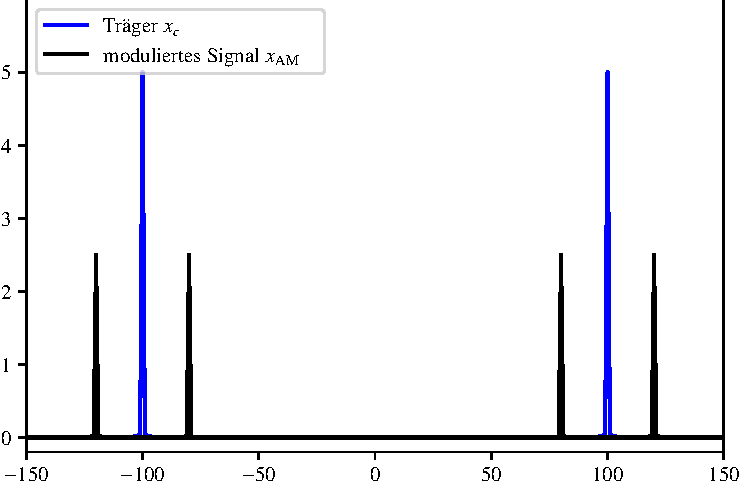
\includegraphics{papers/fm/images/amfrequency.pdf}
	%%% Creator: Matplotlib, PGF backend
%%
%% To include the figure in your LaTeX document, write
%%   \input{<filename>.pgf}
%%
%% Make sure the required packages are loaded in your preamble
%%   \usepackage{pgf}
%%
%% Also ensure that all the required font packages are loaded; for instance,
%% the lmodern package is sometimes necessary when using math font.
%%   \usepackage{lmodern}
%%
%% Figures using additional raster images can only be included by \input if
%% they are in the same directory as the main LaTeX file. For loading figures
%% from other directories you can use the `import` package
%%   \usepackage{import}
%%
%% and then include the figures with
%%   \import{<path to file>}{<filename>.pgf}
%%
%% Matplotlib used the following preamble
%%
\begingroup%
\makeatletter%
\begin{pgfpicture}%
\pgfpathrectangle{\pgfpointorigin}{\pgfqpoint{6.000000in}{4.000000in}}%
\pgfusepath{use as bounding box, clip}%
\begin{pgfscope}%
\pgfsetbuttcap%
\pgfsetmiterjoin%
\pgfsetlinewidth{0.000000pt}%
\definecolor{currentstroke}{rgb}{1.000000,1.000000,1.000000}%
\pgfsetstrokecolor{currentstroke}%
\pgfsetstrokeopacity{0.000000}%
\pgfsetdash{}{0pt}%
\pgfpathmoveto{\pgfqpoint{0.000000in}{0.000000in}}%
\pgfpathlineto{\pgfqpoint{6.000000in}{0.000000in}}%
\pgfpathlineto{\pgfqpoint{6.000000in}{4.000000in}}%
\pgfpathlineto{\pgfqpoint{0.000000in}{4.000000in}}%
\pgfpathlineto{\pgfqpoint{0.000000in}{0.000000in}}%
\pgfpathclose%
\pgfusepath{}%
\end{pgfscope}%
\begin{pgfscope}%
\pgfsetbuttcap%
\pgfsetmiterjoin%
\definecolor{currentfill}{rgb}{1.000000,1.000000,1.000000}%
\pgfsetfillcolor{currentfill}%
\pgfsetlinewidth{0.000000pt}%
\definecolor{currentstroke}{rgb}{0.000000,0.000000,0.000000}%
\pgfsetstrokecolor{currentstroke}%
\pgfsetstrokeopacity{0.000000}%
\pgfsetdash{}{0pt}%
\pgfpathmoveto{\pgfqpoint{0.750000in}{0.500000in}}%
\pgfpathlineto{\pgfqpoint{5.400000in}{0.500000in}}%
\pgfpathlineto{\pgfqpoint{5.400000in}{3.520000in}}%
\pgfpathlineto{\pgfqpoint{0.750000in}{3.520000in}}%
\pgfpathlineto{\pgfqpoint{0.750000in}{0.500000in}}%
\pgfpathclose%
\pgfusepath{fill}%
\end{pgfscope}%
\begin{pgfscope}%
\pgfsetbuttcap%
\pgfsetroundjoin%
\definecolor{currentfill}{rgb}{0.000000,0.000000,0.000000}%
\pgfsetfillcolor{currentfill}%
\pgfsetlinewidth{0.803000pt}%
\definecolor{currentstroke}{rgb}{0.000000,0.000000,0.000000}%
\pgfsetstrokecolor{currentstroke}%
\pgfsetdash{}{0pt}%
\pgfsys@defobject{currentmarker}{\pgfqpoint{0.000000in}{-0.048611in}}{\pgfqpoint{0.000000in}{0.000000in}}{%
\pgfpathmoveto{\pgfqpoint{0.000000in}{0.000000in}}%
\pgfpathlineto{\pgfqpoint{0.000000in}{-0.048611in}}%
\pgfusepath{stroke,fill}%
}%
\begin{pgfscope}%
\pgfsys@transformshift{0.750000in}{0.500000in}%
\pgfsys@useobject{currentmarker}{}%
\end{pgfscope}%
\end{pgfscope}%
\begin{pgfscope}%
\definecolor{textcolor}{rgb}{0.000000,0.000000,0.000000}%
\pgfsetstrokecolor{textcolor}%
\pgfsetfillcolor{textcolor}%
\pgftext[x=0.750000in,y=0.402778in,,top]{\color{textcolor}\rmfamily\fontsize{10.000000}{12.000000}\selectfont \(\displaystyle {\ensuremath{-}150}\)}%
\end{pgfscope}%
\begin{pgfscope}%
\pgfsetbuttcap%
\pgfsetroundjoin%
\definecolor{currentfill}{rgb}{0.000000,0.000000,0.000000}%
\pgfsetfillcolor{currentfill}%
\pgfsetlinewidth{0.803000pt}%
\definecolor{currentstroke}{rgb}{0.000000,0.000000,0.000000}%
\pgfsetstrokecolor{currentstroke}%
\pgfsetdash{}{0pt}%
\pgfsys@defobject{currentmarker}{\pgfqpoint{0.000000in}{-0.048611in}}{\pgfqpoint{0.000000in}{0.000000in}}{%
\pgfpathmoveto{\pgfqpoint{0.000000in}{0.000000in}}%
\pgfpathlineto{\pgfqpoint{0.000000in}{-0.048611in}}%
\pgfusepath{stroke,fill}%
}%
\begin{pgfscope}%
\pgfsys@transformshift{1.525000in}{0.500000in}%
\pgfsys@useobject{currentmarker}{}%
\end{pgfscope}%
\end{pgfscope}%
\begin{pgfscope}%
\definecolor{textcolor}{rgb}{0.000000,0.000000,0.000000}%
\pgfsetstrokecolor{textcolor}%
\pgfsetfillcolor{textcolor}%
\pgftext[x=1.525000in,y=0.402778in,,top]{\color{textcolor}\rmfamily\fontsize{10.000000}{12.000000}\selectfont \(\displaystyle {\ensuremath{-}100}\)}%
\end{pgfscope}%
\begin{pgfscope}%
\pgfsetbuttcap%
\pgfsetroundjoin%
\definecolor{currentfill}{rgb}{0.000000,0.000000,0.000000}%
\pgfsetfillcolor{currentfill}%
\pgfsetlinewidth{0.803000pt}%
\definecolor{currentstroke}{rgb}{0.000000,0.000000,0.000000}%
\pgfsetstrokecolor{currentstroke}%
\pgfsetdash{}{0pt}%
\pgfsys@defobject{currentmarker}{\pgfqpoint{0.000000in}{-0.048611in}}{\pgfqpoint{0.000000in}{0.000000in}}{%
\pgfpathmoveto{\pgfqpoint{0.000000in}{0.000000in}}%
\pgfpathlineto{\pgfqpoint{0.000000in}{-0.048611in}}%
\pgfusepath{stroke,fill}%
}%
\begin{pgfscope}%
\pgfsys@transformshift{2.300000in}{0.500000in}%
\pgfsys@useobject{currentmarker}{}%
\end{pgfscope}%
\end{pgfscope}%
\begin{pgfscope}%
\definecolor{textcolor}{rgb}{0.000000,0.000000,0.000000}%
\pgfsetstrokecolor{textcolor}%
\pgfsetfillcolor{textcolor}%
\pgftext[x=2.300000in,y=0.402778in,,top]{\color{textcolor}\rmfamily\fontsize{10.000000}{12.000000}\selectfont \(\displaystyle {\ensuremath{-}50}\)}%
\end{pgfscope}%
\begin{pgfscope}%
\pgfsetbuttcap%
\pgfsetroundjoin%
\definecolor{currentfill}{rgb}{0.000000,0.000000,0.000000}%
\pgfsetfillcolor{currentfill}%
\pgfsetlinewidth{0.803000pt}%
\definecolor{currentstroke}{rgb}{0.000000,0.000000,0.000000}%
\pgfsetstrokecolor{currentstroke}%
\pgfsetdash{}{0pt}%
\pgfsys@defobject{currentmarker}{\pgfqpoint{0.000000in}{-0.048611in}}{\pgfqpoint{0.000000in}{0.000000in}}{%
\pgfpathmoveto{\pgfqpoint{0.000000in}{0.000000in}}%
\pgfpathlineto{\pgfqpoint{0.000000in}{-0.048611in}}%
\pgfusepath{stroke,fill}%
}%
\begin{pgfscope}%
\pgfsys@transformshift{3.075000in}{0.500000in}%
\pgfsys@useobject{currentmarker}{}%
\end{pgfscope}%
\end{pgfscope}%
\begin{pgfscope}%
\definecolor{textcolor}{rgb}{0.000000,0.000000,0.000000}%
\pgfsetstrokecolor{textcolor}%
\pgfsetfillcolor{textcolor}%
\pgftext[x=3.075000in,y=0.402778in,,top]{\color{textcolor}\rmfamily\fontsize{10.000000}{12.000000}\selectfont \(\displaystyle {0}\)}%
\end{pgfscope}%
\begin{pgfscope}%
\pgfsetbuttcap%
\pgfsetroundjoin%
\definecolor{currentfill}{rgb}{0.000000,0.000000,0.000000}%
\pgfsetfillcolor{currentfill}%
\pgfsetlinewidth{0.803000pt}%
\definecolor{currentstroke}{rgb}{0.000000,0.000000,0.000000}%
\pgfsetstrokecolor{currentstroke}%
\pgfsetdash{}{0pt}%
\pgfsys@defobject{currentmarker}{\pgfqpoint{0.000000in}{-0.048611in}}{\pgfqpoint{0.000000in}{0.000000in}}{%
\pgfpathmoveto{\pgfqpoint{0.000000in}{0.000000in}}%
\pgfpathlineto{\pgfqpoint{0.000000in}{-0.048611in}}%
\pgfusepath{stroke,fill}%
}%
\begin{pgfscope}%
\pgfsys@transformshift{3.850000in}{0.500000in}%
\pgfsys@useobject{currentmarker}{}%
\end{pgfscope}%
\end{pgfscope}%
\begin{pgfscope}%
\definecolor{textcolor}{rgb}{0.000000,0.000000,0.000000}%
\pgfsetstrokecolor{textcolor}%
\pgfsetfillcolor{textcolor}%
\pgftext[x=3.850000in,y=0.402778in,,top]{\color{textcolor}\rmfamily\fontsize{10.000000}{12.000000}\selectfont \(\displaystyle {50}\)}%
\end{pgfscope}%
\begin{pgfscope}%
\pgfsetbuttcap%
\pgfsetroundjoin%
\definecolor{currentfill}{rgb}{0.000000,0.000000,0.000000}%
\pgfsetfillcolor{currentfill}%
\pgfsetlinewidth{0.803000pt}%
\definecolor{currentstroke}{rgb}{0.000000,0.000000,0.000000}%
\pgfsetstrokecolor{currentstroke}%
\pgfsetdash{}{0pt}%
\pgfsys@defobject{currentmarker}{\pgfqpoint{0.000000in}{-0.048611in}}{\pgfqpoint{0.000000in}{0.000000in}}{%
\pgfpathmoveto{\pgfqpoint{0.000000in}{0.000000in}}%
\pgfpathlineto{\pgfqpoint{0.000000in}{-0.048611in}}%
\pgfusepath{stroke,fill}%
}%
\begin{pgfscope}%
\pgfsys@transformshift{4.625000in}{0.500000in}%
\pgfsys@useobject{currentmarker}{}%
\end{pgfscope}%
\end{pgfscope}%
\begin{pgfscope}%
\definecolor{textcolor}{rgb}{0.000000,0.000000,0.000000}%
\pgfsetstrokecolor{textcolor}%
\pgfsetfillcolor{textcolor}%
\pgftext[x=4.625000in,y=0.402778in,,top]{\color{textcolor}\rmfamily\fontsize{10.000000}{12.000000}\selectfont \(\displaystyle {100}\)}%
\end{pgfscope}%
\begin{pgfscope}%
\pgfsetbuttcap%
\pgfsetroundjoin%
\definecolor{currentfill}{rgb}{0.000000,0.000000,0.000000}%
\pgfsetfillcolor{currentfill}%
\pgfsetlinewidth{0.803000pt}%
\definecolor{currentstroke}{rgb}{0.000000,0.000000,0.000000}%
\pgfsetstrokecolor{currentstroke}%
\pgfsetdash{}{0pt}%
\pgfsys@defobject{currentmarker}{\pgfqpoint{0.000000in}{-0.048611in}}{\pgfqpoint{0.000000in}{0.000000in}}{%
\pgfpathmoveto{\pgfqpoint{0.000000in}{0.000000in}}%
\pgfpathlineto{\pgfqpoint{0.000000in}{-0.048611in}}%
\pgfusepath{stroke,fill}%
}%
\begin{pgfscope}%
\pgfsys@transformshift{5.400000in}{0.500000in}%
\pgfsys@useobject{currentmarker}{}%
\end{pgfscope}%
\end{pgfscope}%
\begin{pgfscope}%
\definecolor{textcolor}{rgb}{0.000000,0.000000,0.000000}%
\pgfsetstrokecolor{textcolor}%
\pgfsetfillcolor{textcolor}%
\pgftext[x=5.400000in,y=0.402778in,,top]{\color{textcolor}\rmfamily\fontsize{10.000000}{12.000000}\selectfont \(\displaystyle {150}\)}%
\end{pgfscope}%
\begin{pgfscope}%
\definecolor{textcolor}{rgb}{0.000000,0.000000,0.000000}%
\pgfsetstrokecolor{textcolor}%
\pgfsetfillcolor{textcolor}%
\pgftext[x=3.075000in,y=0.223766in,,top]{\color{textcolor}\rmfamily\fontsize{10.000000}{12.000000}\selectfont Frequency}%
\end{pgfscope}%
\begin{pgfscope}%
\pgfsetbuttcap%
\pgfsetroundjoin%
\definecolor{currentfill}{rgb}{0.000000,0.000000,0.000000}%
\pgfsetfillcolor{currentfill}%
\pgfsetlinewidth{0.803000pt}%
\definecolor{currentstroke}{rgb}{0.000000,0.000000,0.000000}%
\pgfsetstrokecolor{currentstroke}%
\pgfsetdash{}{0pt}%
\pgfsys@defobject{currentmarker}{\pgfqpoint{-0.048611in}{0.000000in}}{\pgfqpoint{-0.000000in}{0.000000in}}{%
\pgfpathmoveto{\pgfqpoint{-0.000000in}{0.000000in}}%
\pgfpathlineto{\pgfqpoint{-0.048611in}{0.000000in}}%
\pgfusepath{stroke,fill}%
}%
\begin{pgfscope}%
\pgfsys@transformshift{0.750000in}{0.597419in}%
\pgfsys@useobject{currentmarker}{}%
\end{pgfscope}%
\end{pgfscope}%
\begin{pgfscope}%
\definecolor{textcolor}{rgb}{0.000000,0.000000,0.000000}%
\pgfsetstrokecolor{textcolor}%
\pgfsetfillcolor{textcolor}%
\pgftext[x=0.475308in, y=0.549194in, left, base]{\color{textcolor}\rmfamily\fontsize{10.000000}{12.000000}\selectfont \(\displaystyle {0.0}\)}%
\end{pgfscope}%
\begin{pgfscope}%
\pgfsetbuttcap%
\pgfsetroundjoin%
\definecolor{currentfill}{rgb}{0.000000,0.000000,0.000000}%
\pgfsetfillcolor{currentfill}%
\pgfsetlinewidth{0.803000pt}%
\definecolor{currentstroke}{rgb}{0.000000,0.000000,0.000000}%
\pgfsetstrokecolor{currentstroke}%
\pgfsetdash{}{0pt}%
\pgfsys@defobject{currentmarker}{\pgfqpoint{-0.048611in}{0.000000in}}{\pgfqpoint{-0.000000in}{0.000000in}}{%
\pgfpathmoveto{\pgfqpoint{-0.000000in}{0.000000in}}%
\pgfpathlineto{\pgfqpoint{-0.048611in}{0.000000in}}%
\pgfusepath{stroke,fill}%
}%
\begin{pgfscope}%
\pgfsys@transformshift{0.750000in}{1.084516in}%
\pgfsys@useobject{currentmarker}{}%
\end{pgfscope}%
\end{pgfscope}%
\begin{pgfscope}%
\definecolor{textcolor}{rgb}{0.000000,0.000000,0.000000}%
\pgfsetstrokecolor{textcolor}%
\pgfsetfillcolor{textcolor}%
\pgftext[x=0.475308in, y=1.036291in, left, base]{\color{textcolor}\rmfamily\fontsize{10.000000}{12.000000}\selectfont \(\displaystyle {0.1}\)}%
\end{pgfscope}%
\begin{pgfscope}%
\pgfsetbuttcap%
\pgfsetroundjoin%
\definecolor{currentfill}{rgb}{0.000000,0.000000,0.000000}%
\pgfsetfillcolor{currentfill}%
\pgfsetlinewidth{0.803000pt}%
\definecolor{currentstroke}{rgb}{0.000000,0.000000,0.000000}%
\pgfsetstrokecolor{currentstroke}%
\pgfsetdash{}{0pt}%
\pgfsys@defobject{currentmarker}{\pgfqpoint{-0.048611in}{0.000000in}}{\pgfqpoint{-0.000000in}{0.000000in}}{%
\pgfpathmoveto{\pgfqpoint{-0.000000in}{0.000000in}}%
\pgfpathlineto{\pgfqpoint{-0.048611in}{0.000000in}}%
\pgfusepath{stroke,fill}%
}%
\begin{pgfscope}%
\pgfsys@transformshift{0.750000in}{1.571613in}%
\pgfsys@useobject{currentmarker}{}%
\end{pgfscope}%
\end{pgfscope}%
\begin{pgfscope}%
\definecolor{textcolor}{rgb}{0.000000,0.000000,0.000000}%
\pgfsetstrokecolor{textcolor}%
\pgfsetfillcolor{textcolor}%
\pgftext[x=0.475308in, y=1.523388in, left, base]{\color{textcolor}\rmfamily\fontsize{10.000000}{12.000000}\selectfont \(\displaystyle {0.2}\)}%
\end{pgfscope}%
\begin{pgfscope}%
\pgfsetbuttcap%
\pgfsetroundjoin%
\definecolor{currentfill}{rgb}{0.000000,0.000000,0.000000}%
\pgfsetfillcolor{currentfill}%
\pgfsetlinewidth{0.803000pt}%
\definecolor{currentstroke}{rgb}{0.000000,0.000000,0.000000}%
\pgfsetstrokecolor{currentstroke}%
\pgfsetdash{}{0pt}%
\pgfsys@defobject{currentmarker}{\pgfqpoint{-0.048611in}{0.000000in}}{\pgfqpoint{-0.000000in}{0.000000in}}{%
\pgfpathmoveto{\pgfqpoint{-0.000000in}{0.000000in}}%
\pgfpathlineto{\pgfqpoint{-0.048611in}{0.000000in}}%
\pgfusepath{stroke,fill}%
}%
\begin{pgfscope}%
\pgfsys@transformshift{0.750000in}{2.058710in}%
\pgfsys@useobject{currentmarker}{}%
\end{pgfscope}%
\end{pgfscope}%
\begin{pgfscope}%
\definecolor{textcolor}{rgb}{0.000000,0.000000,0.000000}%
\pgfsetstrokecolor{textcolor}%
\pgfsetfillcolor{textcolor}%
\pgftext[x=0.475308in, y=2.010484in, left, base]{\color{textcolor}\rmfamily\fontsize{10.000000}{12.000000}\selectfont \(\displaystyle {0.3}\)}%
\end{pgfscope}%
\begin{pgfscope}%
\pgfsetbuttcap%
\pgfsetroundjoin%
\definecolor{currentfill}{rgb}{0.000000,0.000000,0.000000}%
\pgfsetfillcolor{currentfill}%
\pgfsetlinewidth{0.803000pt}%
\definecolor{currentstroke}{rgb}{0.000000,0.000000,0.000000}%
\pgfsetstrokecolor{currentstroke}%
\pgfsetdash{}{0pt}%
\pgfsys@defobject{currentmarker}{\pgfqpoint{-0.048611in}{0.000000in}}{\pgfqpoint{-0.000000in}{0.000000in}}{%
\pgfpathmoveto{\pgfqpoint{-0.000000in}{0.000000in}}%
\pgfpathlineto{\pgfqpoint{-0.048611in}{0.000000in}}%
\pgfusepath{stroke,fill}%
}%
\begin{pgfscope}%
\pgfsys@transformshift{0.750000in}{2.545806in}%
\pgfsys@useobject{currentmarker}{}%
\end{pgfscope}%
\end{pgfscope}%
\begin{pgfscope}%
\definecolor{textcolor}{rgb}{0.000000,0.000000,0.000000}%
\pgfsetstrokecolor{textcolor}%
\pgfsetfillcolor{textcolor}%
\pgftext[x=0.475308in, y=2.497581in, left, base]{\color{textcolor}\rmfamily\fontsize{10.000000}{12.000000}\selectfont \(\displaystyle {0.4}\)}%
\end{pgfscope}%
\begin{pgfscope}%
\pgfsetbuttcap%
\pgfsetroundjoin%
\definecolor{currentfill}{rgb}{0.000000,0.000000,0.000000}%
\pgfsetfillcolor{currentfill}%
\pgfsetlinewidth{0.803000pt}%
\definecolor{currentstroke}{rgb}{0.000000,0.000000,0.000000}%
\pgfsetstrokecolor{currentstroke}%
\pgfsetdash{}{0pt}%
\pgfsys@defobject{currentmarker}{\pgfqpoint{-0.048611in}{0.000000in}}{\pgfqpoint{-0.000000in}{0.000000in}}{%
\pgfpathmoveto{\pgfqpoint{-0.000000in}{0.000000in}}%
\pgfpathlineto{\pgfqpoint{-0.048611in}{0.000000in}}%
\pgfusepath{stroke,fill}%
}%
\begin{pgfscope}%
\pgfsys@transformshift{0.750000in}{3.032903in}%
\pgfsys@useobject{currentmarker}{}%
\end{pgfscope}%
\end{pgfscope}%
\begin{pgfscope}%
\definecolor{textcolor}{rgb}{0.000000,0.000000,0.000000}%
\pgfsetstrokecolor{textcolor}%
\pgfsetfillcolor{textcolor}%
\pgftext[x=0.475308in, y=2.984678in, left, base]{\color{textcolor}\rmfamily\fontsize{10.000000}{12.000000}\selectfont \(\displaystyle {0.5}\)}%
\end{pgfscope}%
\begin{pgfscope}%
\definecolor{textcolor}{rgb}{0.000000,0.000000,0.000000}%
\pgfsetstrokecolor{textcolor}%
\pgfsetfillcolor{textcolor}%
\pgftext[x=0.419753in,y=2.010000in,,bottom,rotate=90.000000]{\color{textcolor}\rmfamily\fontsize{10.000000}{12.000000}\selectfont Magnetude}%
\end{pgfscope}%
\begin{pgfscope}%
\pgfpathrectangle{\pgfqpoint{0.750000in}{0.500000in}}{\pgfqpoint{4.650000in}{3.020000in}}%
\pgfusepath{clip}%
\pgfsetrectcap%
\pgfsetroundjoin%
\pgfsetlinewidth{1.505625pt}%
\definecolor{currentstroke}{rgb}{0.000000,0.000000,1.000000}%
\pgfsetstrokecolor{currentstroke}%
\pgfsetdash{}{0pt}%
\pgfpathmoveto{\pgfqpoint{3.075000in}{0.597906in}}%
\pgfpathlineto{\pgfqpoint{4.423500in}{0.599422in}}%
\pgfpathlineto{\pgfqpoint{4.532000in}{0.601597in}}%
\pgfpathlineto{\pgfqpoint{4.563000in}{0.603617in}}%
\pgfpathlineto{\pgfqpoint{4.578500in}{0.605634in}}%
\pgfpathlineto{\pgfqpoint{4.594000in}{0.609658in}}%
\pgfpathlineto{\pgfqpoint{4.609500in}{0.621654in}}%
\pgfpathlineto{\pgfqpoint{4.625000in}{3.032624in}}%
\pgfpathlineto{\pgfqpoint{4.640500in}{0.621897in}}%
\pgfpathlineto{\pgfqpoint{4.656000in}{0.609537in}}%
\pgfpathlineto{\pgfqpoint{4.671500in}{0.605444in}}%
\pgfpathlineto{\pgfqpoint{4.702500in}{0.602181in}}%
\pgfpathlineto{\pgfqpoint{4.764500in}{0.600012in}}%
\pgfpathlineto{\pgfqpoint{4.935000in}{0.598527in}}%
\pgfpathlineto{\pgfqpoint{5.413889in}{0.597801in}}%
\pgfpathmoveto{\pgfqpoint{5.413889in}{0.597419in}}%
\pgfpathlineto{\pgfqpoint{0.736111in}{0.597419in}}%
\pgfpathmoveto{\pgfqpoint{0.736111in}{0.597801in}}%
\pgfpathlineto{\pgfqpoint{1.354500in}{0.599520in}}%
\pgfpathlineto{\pgfqpoint{1.447500in}{0.602181in}}%
\pgfpathlineto{\pgfqpoint{1.478500in}{0.605444in}}%
\pgfpathlineto{\pgfqpoint{1.494000in}{0.609537in}}%
\pgfpathlineto{\pgfqpoint{1.509500in}{0.621897in}}%
\pgfpathlineto{\pgfqpoint{1.525000in}{3.032624in}}%
\pgfpathlineto{\pgfqpoint{1.540500in}{0.621654in}}%
\pgfpathlineto{\pgfqpoint{1.556000in}{0.609658in}}%
\pgfpathlineto{\pgfqpoint{1.571500in}{0.605634in}}%
\pgfpathlineto{\pgfqpoint{1.602500in}{0.602405in}}%
\pgfpathlineto{\pgfqpoint{1.664500in}{0.600250in}}%
\pgfpathlineto{\pgfqpoint{1.835000in}{0.598772in}}%
\pgfpathlineto{\pgfqpoint{2.455000in}{0.597999in}}%
\pgfpathlineto{\pgfqpoint{3.059500in}{0.597907in}}%
\pgfpathlineto{\pgfqpoint{3.059500in}{0.597907in}}%
\pgfusepath{stroke}%
\end{pgfscope}%
\begin{pgfscope}%
\pgfpathrectangle{\pgfqpoint{0.750000in}{0.500000in}}{\pgfqpoint{4.650000in}{3.020000in}}%
\pgfusepath{clip}%
\pgfsetrectcap%
\pgfsetroundjoin%
\pgfsetlinewidth{1.505625pt}%
\definecolor{currentstroke}{rgb}{0.000000,0.000000,0.000000}%
\pgfsetstrokecolor{currentstroke}%
\pgfsetdash{}{0pt}%
\pgfpathmoveto{\pgfqpoint{3.075000in}{0.597570in}}%
\pgfpathlineto{\pgfqpoint{4.222000in}{0.598826in}}%
\pgfpathlineto{\pgfqpoint{4.268500in}{0.600416in}}%
\pgfpathlineto{\pgfqpoint{4.284000in}{0.602020in}}%
\pgfpathlineto{\pgfqpoint{4.299500in}{0.606823in}}%
\pgfpathlineto{\pgfqpoint{4.315000in}{1.814761in}}%
\pgfpathlineto{\pgfqpoint{4.330500in}{0.607522in}}%
\pgfpathlineto{\pgfqpoint{4.346000in}{0.602604in}}%
\pgfpathlineto{\pgfqpoint{4.377000in}{0.600178in}}%
\pgfpathlineto{\pgfqpoint{4.470000in}{0.598802in}}%
\pgfpathlineto{\pgfqpoint{4.749000in}{0.598927in}}%
\pgfpathlineto{\pgfqpoint{4.857500in}{0.600562in}}%
\pgfpathlineto{\pgfqpoint{4.888500in}{0.602484in}}%
\pgfpathlineto{\pgfqpoint{4.904000in}{0.604889in}}%
\pgfpathlineto{\pgfqpoint{4.919500in}{0.612059in}}%
\pgfpathlineto{\pgfqpoint{4.935000in}{1.815069in}}%
\pgfpathlineto{\pgfqpoint{4.950500in}{0.612016in}}%
\pgfpathlineto{\pgfqpoint{4.966000in}{0.604583in}}%
\pgfpathlineto{\pgfqpoint{4.997000in}{0.600906in}}%
\pgfpathlineto{\pgfqpoint{5.059000in}{0.599087in}}%
\pgfpathlineto{\pgfqpoint{5.260500in}{0.597991in}}%
\pgfpathlineto{\pgfqpoint{5.413889in}{0.597786in}}%
\pgfpathmoveto{\pgfqpoint{5.413889in}{0.597422in}}%
\pgfpathlineto{\pgfqpoint{0.736111in}{0.597422in}}%
\pgfpathmoveto{\pgfqpoint{0.736111in}{0.597786in}}%
\pgfpathlineto{\pgfqpoint{1.106500in}{0.599345in}}%
\pgfpathlineto{\pgfqpoint{1.168500in}{0.602128in}}%
\pgfpathlineto{\pgfqpoint{1.184000in}{0.604583in}}%
\pgfpathlineto{\pgfqpoint{1.199500in}{0.612016in}}%
\pgfpathlineto{\pgfqpoint{1.215000in}{1.815069in}}%
\pgfpathlineto{\pgfqpoint{1.230500in}{0.612059in}}%
\pgfpathlineto{\pgfqpoint{1.246000in}{0.604889in}}%
\pgfpathlineto{\pgfqpoint{1.277000in}{0.601282in}}%
\pgfpathlineto{\pgfqpoint{1.339000in}{0.599494in}}%
\pgfpathlineto{\pgfqpoint{1.525000in}{0.598571in}}%
\pgfpathlineto{\pgfqpoint{1.757500in}{0.599702in}}%
\pgfpathlineto{\pgfqpoint{1.804000in}{0.602604in}}%
\pgfpathlineto{\pgfqpoint{1.819500in}{0.607522in}}%
\pgfpathlineto{\pgfqpoint{1.835000in}{1.814761in}}%
\pgfpathlineto{\pgfqpoint{1.850500in}{0.606823in}}%
\pgfpathlineto{\pgfqpoint{1.866000in}{0.602020in}}%
\pgfpathlineto{\pgfqpoint{1.897000in}{0.599618in}}%
\pgfpathlineto{\pgfqpoint{1.990000in}{0.598209in}}%
\pgfpathlineto{\pgfqpoint{2.393000in}{0.597632in}}%
\pgfpathlineto{\pgfqpoint{3.059500in}{0.597570in}}%
\pgfpathlineto{\pgfqpoint{3.059500in}{0.597570in}}%
\pgfusepath{stroke}%
\end{pgfscope}%
\begin{pgfscope}%
\pgfsetrectcap%
\pgfsetmiterjoin%
\pgfsetlinewidth{0.803000pt}%
\definecolor{currentstroke}{rgb}{0.000000,0.000000,0.000000}%
\pgfsetstrokecolor{currentstroke}%
\pgfsetdash{}{0pt}%
\pgfpathmoveto{\pgfqpoint{0.750000in}{0.500000in}}%
\pgfpathlineto{\pgfqpoint{0.750000in}{3.520000in}}%
\pgfusepath{stroke}%
\end{pgfscope}%
\begin{pgfscope}%
\pgfsetrectcap%
\pgfsetmiterjoin%
\pgfsetlinewidth{0.803000pt}%
\definecolor{currentstroke}{rgb}{0.000000,0.000000,0.000000}%
\pgfsetstrokecolor{currentstroke}%
\pgfsetdash{}{0pt}%
\pgfpathmoveto{\pgfqpoint{5.400000in}{0.500000in}}%
\pgfpathlineto{\pgfqpoint{5.400000in}{3.520000in}}%
\pgfusepath{stroke}%
\end{pgfscope}%
\begin{pgfscope}%
\pgfsetrectcap%
\pgfsetmiterjoin%
\pgfsetlinewidth{0.803000pt}%
\definecolor{currentstroke}{rgb}{0.000000,0.000000,0.000000}%
\pgfsetstrokecolor{currentstroke}%
\pgfsetdash{}{0pt}%
\pgfpathmoveto{\pgfqpoint{0.750000in}{0.500000in}}%
\pgfpathlineto{\pgfqpoint{5.400000in}{0.500000in}}%
\pgfusepath{stroke}%
\end{pgfscope}%
\begin{pgfscope}%
\pgfsetrectcap%
\pgfsetmiterjoin%
\pgfsetlinewidth{0.803000pt}%
\definecolor{currentstroke}{rgb}{0.000000,0.000000,0.000000}%
\pgfsetstrokecolor{currentstroke}%
\pgfsetdash{}{0pt}%
\pgfpathmoveto{\pgfqpoint{0.750000in}{3.520000in}}%
\pgfpathlineto{\pgfqpoint{5.400000in}{3.520000in}}%
\pgfusepath{stroke}%
\end{pgfscope}%
\begin{pgfscope}%
\pgfsetbuttcap%
\pgfsetmiterjoin%
\definecolor{currentfill}{rgb}{1.000000,1.000000,1.000000}%
\pgfsetfillcolor{currentfill}%
\pgfsetfillopacity{0.800000}%
\pgfsetlinewidth{1.003750pt}%
\definecolor{currentstroke}{rgb}{0.800000,0.800000,0.800000}%
\pgfsetstrokecolor{currentstroke}%
\pgfsetstrokeopacity{0.800000}%
\pgfsetdash{}{0pt}%
\pgfpathmoveto{\pgfqpoint{0.847222in}{3.021543in}}%
\pgfpathlineto{\pgfqpoint{2.709417in}{3.021543in}}%
\pgfpathquadraticcurveto{\pgfqpoint{2.737194in}{3.021543in}}{\pgfqpoint{2.737194in}{3.049321in}}%
\pgfpathlineto{\pgfqpoint{2.737194in}{3.422778in}}%
\pgfpathquadraticcurveto{\pgfqpoint{2.737194in}{3.450556in}}{\pgfqpoint{2.709417in}{3.450556in}}%
\pgfpathlineto{\pgfqpoint{0.847222in}{3.450556in}}%
\pgfpathquadraticcurveto{\pgfqpoint{0.819444in}{3.450556in}}{\pgfqpoint{0.819444in}{3.422778in}}%
\pgfpathlineto{\pgfqpoint{0.819444in}{3.049321in}}%
\pgfpathquadraticcurveto{\pgfqpoint{0.819444in}{3.021543in}}{\pgfqpoint{0.847222in}{3.021543in}}%
\pgfpathlineto{\pgfqpoint{0.847222in}{3.021543in}}%
\pgfpathclose%
\pgfusepath{stroke,fill}%
\end{pgfscope}%
\begin{pgfscope}%
\pgfsetrectcap%
\pgfsetroundjoin%
\pgfsetlinewidth{1.505625pt}%
\definecolor{currentstroke}{rgb}{0.000000,0.000000,1.000000}%
\pgfsetstrokecolor{currentstroke}%
\pgfsetdash{}{0pt}%
\pgfpathmoveto{\pgfqpoint{0.875000in}{3.346389in}}%
\pgfpathlineto{\pgfqpoint{1.013889in}{3.346389in}}%
\pgfpathlineto{\pgfqpoint{1.152778in}{3.346389in}}%
\pgfusepath{stroke}%
\end{pgfscope}%
\begin{pgfscope}%
\definecolor{textcolor}{rgb}{0.000000,0.000000,0.000000}%
\pgfsetstrokecolor{textcolor}%
\pgfsetfillcolor{textcolor}%
\pgftext[x=1.263889in,y=3.297778in,left,base]{\color{textcolor}\rmfamily\fontsize{10.000000}{12.000000}\selectfont Träger \(\displaystyle x_c\)}%
\end{pgfscope}%
\begin{pgfscope}%
\pgfsetrectcap%
\pgfsetroundjoin%
\pgfsetlinewidth{1.505625pt}%
\definecolor{currentstroke}{rgb}{0.000000,0.000000,0.000000}%
\pgfsetstrokecolor{currentstroke}%
\pgfsetdash{}{0pt}%
\pgfpathmoveto{\pgfqpoint{0.875000in}{3.152716in}}%
\pgfpathlineto{\pgfqpoint{1.013889in}{3.152716in}}%
\pgfpathlineto{\pgfqpoint{1.152778in}{3.152716in}}%
\pgfusepath{stroke}%
\end{pgfscope}%
\begin{pgfscope}%
\definecolor{textcolor}{rgb}{0.000000,0.000000,0.000000}%
\pgfsetstrokecolor{textcolor}%
\pgfsetfillcolor{textcolor}%
\pgftext[x=1.263889in,y=3.104105in,left,base]{\color{textcolor}\rmfamily\fontsize{10.000000}{12.000000}\selectfont moduiertes Signal \(\displaystyle x_{AM}\)}%
\end{pgfscope}%
\end{pgfpicture}%
\makeatother%
\endgroup%

	\caption{Amplitudenmodulation im Frequenzspektrum}
	\label{fig:AM_frequency}
\end{figure}
Fürs Frequenzmultiplexen wird dann das Signal \(m(t)\) in die verschiedenen Frequenzen unterteilt um mehr Nachrichten zu übertragen.
Doch aufs Frequenzmultiplexen und weitere formen wie SSB und DSB möchte ich nicht weiter eingehen.
Diese können gerne im Nat Skript nachgelesen werden.\cite{fm:NAT}

Das sich unser Signal \(m(t)\)  so mit dem Träger Signal verhält findet es man wieder gut beim empfangen, mit Hilfe der Bandbreite weiss man was alles dazugehört.
Bei der Frequenzmodulation ist dies einwenig anders, dies sieht man auch in der Abb. \ref{fig:fm:FM}.
Da in der Frequenzmodulation das Nachrichtensignal \(m(t)\) die Frequenzändert und somit auch im Frequenzbereich nicht mehr einfach bestimmbar ist.
